%!TEX root = main.tex
\subsection{Moment Averaging for the OLS versus 2SLS Example}
Although it is a special case of moment averaging, moment selection is a somewhat crude procedure: it gives full weight to the estimator that minimizes the moment selection criterion no matter how close its nearest competitor lies. 
Accordingly, when competing moment sets have similar criterion values in the population, sampling variation can be \emph{magnified} in the selected estimator. 
Thus, it may be possible to achieve better performance by using smooth weights rather than discrete selection.
In this section, we briefly explore this possibility.

They key question is: how should we construct the weights?
One possibility is to adapt a proposal from \cite{Burnhametal}, who suggest averaging a collection of competing maximum likelihood estimator with weights of the form 
\[w_k =\left. \exp(-I_k/2)\right/\sum_{i=1}^K \exp(-I_i/2)\] 
where $I_k$ is an information criterion evaluated for model $k$, and $i$ indexes the set of $K$ candidate models. 
This expression, constructed by an analogy with Bayesian model averaging, gives more weight to models with lower values of the information criterion but non-zero weight to all models. 
Applying a slightly more general form of this idea, suggested by \cite{ClaeskensHjortbook}, to the moment selection criteria examined above, we might consider using weights of the form	
\[		\widehat{\omega}_S = \left.\exp\left\{-\frac{\kappa}{2} \mbox{MSC}(S)\right\}\right/\sum_{S' \in \mathscr{S}}\exp\left\{-\frac{\kappa}{2} \mbox{MSC}(S')\right\}\]
where MSC$(\cdot)$ is a moment selection criterion and the parameter $\kappa \geq 0$ varies the uniformity of the weighting. 
As $\kappa \rightarrow 0$ the weights become more uniform; as $\kappa \rightarrow \infty$ they approach the moment selection procedure given by minimizing the corresponding criterion. 
Setting $\kappa = 1$ gives the \cite{Burnhametal} weights.

Some preliminary simulation results, reported in an earlier draft of this paper, suggest that exponential weighting can indeed provide MSE improvements, so long as we choose an appropriate value for $\kappa$.
And there's the rub: while it is easy to experiment with different values of $\kappa$ in a simulation study, it is far from clear how to set about formulating a rule to choose $\kappa$ in practice. In at least some applications, however, there is a compelling alternative to the exponential weighting scheme: we can instead derive weights \emph{analytically} to minimize AMSE within the FMSC framework.\footnote{I thank Bruce Hansen for suggesting this idea.} 
To illustrate this idea, we revisit the OLS versus 2SLS example from Sections \ref{sec:OLSvsIVlowlevel} and \ref{sec:FMSCforOLSvsIV}. 

To begin, define an arbitrary weighted average of the OLS and 2SLS estimators from Equations \ref{eq:OLS} and \ref{eq:2SLS} by  
\begin{equation}
	\widetilde{\beta}(\omega) = \omega \widehat{\beta}_{OLS} + (1 - \omega) \widetilde{\beta}_{2SLS}
\end{equation}
where $\omega \in [0,1]$ is the weight given to the OLS estimator.
Since the weights sum to one, we have
\begin{eqnarray*}
	\sqrt{n}\left[\widehat{\beta}(\omega) - \beta \right] &=& \left[ \begin{array}
	{cc} \omega & (1 - \omega)
\end{array}\right] \left[
\begin{array}{c}
  \sqrt{n}(\widehat{\beta}_{OLS} - \beta) \\
  \sqrt{n}(\widetilde{\beta}_{2SLS} - \beta)
\end{array}
\right]\\
& \overset{d}{\rightarrow} & N\left(\mbox{Bias}\left[\widehat{\beta}(\omega)\right], Var\left[\widehat{\beta}(\omega)\right] \right)
\end{eqnarray*}
by Theorem \ref{thm:OLSvsIV}, where
\begin{eqnarray*}
	\mbox{Bias}\left[\widehat{\beta}(\omega)\right] &=& \omega \left( \frac{\tau}{\sigma_x^2} \right) \\
	 Var\left[\widehat{\beta}(\omega)\right] &=&  \frac{\sigma_\epsilon^2}{\sigma_x^2} \left[(2\omega^2 - \omega)\left( \frac{\sigma_x^2}{\gamma^2} - 1\right)+\frac{\sigma_x^2}{\gamma^2} \right]
\end{eqnarray*}
and accordingly
\begin{equation}
	\mbox{AMSE}\left[\widehat{\beta}(\omega) \right] =  \omega^2 \left(\frac{\tau^2}{\sigma_x^4} \right) + (\omega^2 - 2 \omega)\left(\frac{\sigma_\epsilon^2}{\sigma_x^2}\right)\left( \frac{\sigma_x^2}{\gamma^2} - 1\right) + \frac{\sigma_\epsilon^2}{\gamma^2}.
\end{equation}
The preceding expression is a globally convex function of $\omega$. 
Taking the first order condition and rearranging, we find that the unique global minimizer is
\begin{equation}
\label{eq:AMSEoptimal}
	\omega^* = \underset{\omega \in [0,1]}{\mbox{arg min}}\; \mbox{AMSE}\left[\widehat{\beta}(\omega) \right] 
	=\left[1 + \frac{\tau^2/\sigma_x^4}{\sigma_\epsilon^2(1/\gamma^2 - 1/\sigma_x^2)}\right]^{-1}
\end{equation}
In other words,
$$\omega^* = \left[1 + \frac{\mbox{ABIAS(OLS)}^2}{\mbox{AVAR(2SLS)}-\mbox{AVAR(OLS)}} \right]^{-1}$$

This expression has several important consequences. 
First, since the variance of the 2SLS estimator is always strictly greater than that of the OLS estimator, the optimal value of $\omega$ \emph{cannot} be zero. 
No matter how strong the endogeneity of $x$ as measured by $\tau$, we should always give some weight to the OLS estimator. 
Second, when $\tau = 0$ the optimal value of $\omega$ is one. If $x$ is exogenous, OLS is strictly preferable to 2SLS. 
Third, the optimal weights depend on the strength of the instruments $\mathbf{z}$ as measured by $\gamma$. 
For a given value of $\tau\neq 0$, the stronger the instruments, the less weight we should give to OLS.

Equation \ref{eq:AMSEoptimal} gives the AMSE-optimal weighted average of the OLS and 2SLS estimators. 
To actually use the corresponding moment average estimator in practice, however, we need to estimate the unknowns.
As discussed above in Section \ref{sec:FMSCforOLSvsIV} the usual estimators of $\sigma_x^2$ and $\gamma$ remain consistent under local mis-specification, and the residuals from the 2SLS estimator provide a robust estimator of $\sigma_\epsilon^2$.
As before, the problem is estimating $\tau^2$.
A natural idea is to substitute the asymptotically unbiased estimator that arises from Theorem \ref{thm:tauOLSvsIV}, namely $\widehat{\tau}^2 - \widehat{V}$. 
The problem with this approach is that, while $\tau^2$ is always greater than or equal to zero as is $\widehat{\tau}^2$, the difference $\widehat{\tau}^2 - \widehat{V}$ can easily be negative, yielding a \emph{negative} estimate of $\mbox{ABIAS(OLS)}^2$.
To solve this problem, we borrow an idea from the literature on shrinkage estimation and use the \emph{positive part} instead, namely $\max\{0, \; \widehat{\tau}^2 - \widehat{V}\}$, as in the positive-part James-Stein estimator.
This ensures that our estimator of $\omega^*$ lies inside the interval $[0,1]$.
Accordingly, we define 
\begin{equation}
	\widehat{\beta}^*_{AVG} = \widehat{\omega}^* \widehat{\beta}_{OLS} + (1 - \widehat{\omega}^*)\widetilde{\beta}_{2SLS}
	\label{eq:OLSvsIV_AVG1}
\end{equation}
where
\begin{equation}
\widehat{\omega }^* = \left[1 + \frac{\max \left\{0, \; \left(\widehat{\tau}^2 - \widehat{\sigma}_\epsilon^2\widehat{\sigma}_x^2  \left(\widehat{\sigma}_x^2/\widehat{\gamma}^2 - 1 \right) \right)/\;\widehat{\sigma}_x^4 \right\}}{\widehat{\sigma}_\epsilon^2 (1/\widehat{\gamma}^2 - 1/\widehat{\sigma}_x^2)}\right]^{-1}
	\label{eq:OLSvsIV_AVG2}
\end{equation}

Returning to the simulation experiment from Section \ref{sec:OLSvsIVsim}, Figure \ref{fig:OLSvsIV_AVG} compares the finite-sample RMSE of the minimum-AMSE moment average estimator presented in Equations \ref{eq:OLSvsIV_AVG1} and \ref{eq:OLSvsIV_AVG2} to those of the FMSC and DHW pre-test estimators from Figure \ref{fig:OLSvsIV_RMSEvsDHW}.
The performance of the minimum-AMSE moment average estimator is strong: it provides the lowest worst-case RMSE and improves uniformly on the FMSC for all but the largest values of $\rho$.
While a complete examination of minimum-AMSE moment averaging is beyond the scope of the present paper, these results suggest that it could prove extremely useful in practice.
In the following section we will see how to construct a valid confidence interval for this and related procedures.
\begin{figure}
\centering
	% Created by tikzDevice version 0.7.0 on 2014-07-01 19:29:03
% !TEX encoding = UTF-8 Unicode
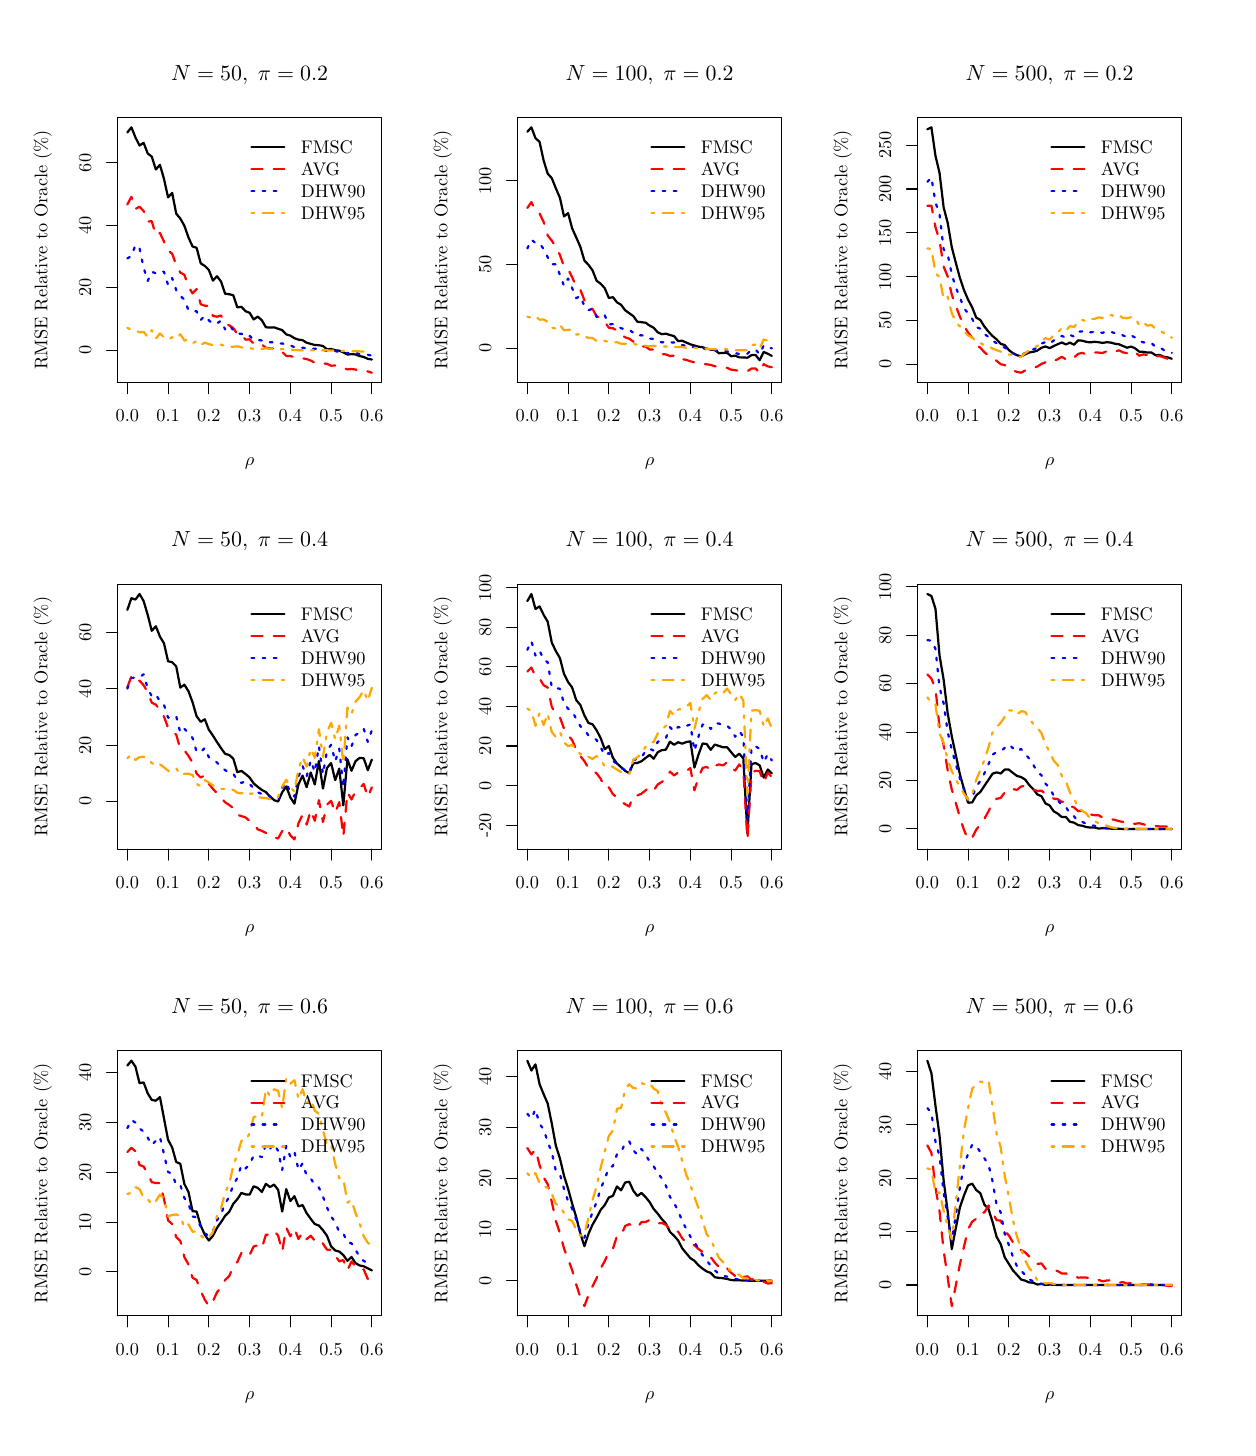
\begin{tikzpicture}[x=1pt,y=1pt]
\definecolor[named]{fillColor}{rgb}{1.00,1.00,1.00}
\path[use as bounding box,fill=fillColor,fill opacity=0.00] (0,0) rectangle (433.62,505.89);
\begin{scope}
\path[clip] ( 32.47,377.65) rectangle (127.91,473.42);
\definecolor[named]{drawColor}{rgb}{0.00,0.00,0.00}

\path[draw=drawColor,line width= 0.8pt,line join=round,line cap=round] ( 36.01,468.01) --
	( 37.48,469.87) --
	( 38.95,466.21) --
	( 40.42,463.29) --
	( 41.90,464.28) --
	( 43.37,460.43) --
	( 44.84,459.29) --
	( 46.32,454.63) --
	( 47.79,456.33) --
	( 49.26,451.21) --
	( 50.73,444.55) --
	( 52.21,446.18) --
	( 53.68,438.68) --
	( 55.15,436.91) --
	( 56.63,434.30) --
	( 58.10,430.10) --
	( 59.57,426.83) --
	( 61.04,426.35) --
	( 62.52,420.75) --
	( 63.99,419.80) --
	( 65.46,418.35) --
	( 66.93,414.49) --
	( 68.41,416.06) --
	( 69.88,414.12) --
	( 71.35,409.77) --
	( 72.83,409.56) --
	( 74.30,409.21) --
	( 75.77,404.81) --
	( 77.24,405.02) --
	( 78.72,403.44) --
	( 80.19,402.86) --
	( 81.66,400.46) --
	( 83.14,401.48) --
	( 84.61,400.16) --
	( 86.08,397.63) --
	( 87.55,397.50) --
	( 89.03,397.60) --
	( 90.50,397.10) --
	( 91.97,396.59) --
	( 93.44,395.05) --
	( 94.92,394.60) --
	( 96.39,393.68) --
	( 97.86,393.17) --
	( 99.34,392.96) --
	(100.81,392.04) --
	(102.28,391.63) --
	(103.75,391.21) --
	(105.23,391.15) --
	(106.70,390.86) --
	(108.17,389.69) --
	(109.65,389.78) --
	(111.12,389.32) --
	(112.59,389.17) --
	(114.06,388.58) --
	(115.54,387.75) --
	(117.01,387.93) --
	(118.48,387.80) --
	(119.95,387.22) --
	(121.43,386.90) --
	(122.90,386.22) --
	(124.37,385.98);
\end{scope}
\begin{scope}
\path[clip] (  0.00,  0.00) rectangle (433.62,505.89);
\definecolor[named]{drawColor}{rgb}{0.00,0.00,0.00}

\path[draw=drawColor,line width= 0.4pt,line join=round,line cap=round] ( 36.01,377.65) -- (124.37,377.65);

\path[draw=drawColor,line width= 0.4pt,line join=round,line cap=round] ( 36.01,377.65) -- ( 36.01,373.69);

\path[draw=drawColor,line width= 0.4pt,line join=round,line cap=round] ( 50.73,377.65) -- ( 50.73,373.69);

\path[draw=drawColor,line width= 0.4pt,line join=round,line cap=round] ( 65.46,377.65) -- ( 65.46,373.69);

\path[draw=drawColor,line width= 0.4pt,line join=round,line cap=round] ( 80.19,377.65) -- ( 80.19,373.69);

\path[draw=drawColor,line width= 0.4pt,line join=round,line cap=round] ( 94.92,377.65) -- ( 94.92,373.69);

\path[draw=drawColor,line width= 0.4pt,line join=round,line cap=round] (109.65,377.65) -- (109.65,373.69);

\path[draw=drawColor,line width= 0.4pt,line join=round,line cap=round] (124.37,377.65) -- (124.37,373.69);

\node[text=drawColor,anchor=base,inner sep=0pt, outer sep=0pt, scale=  0.66] at ( 36.01,363.40) {0.0};

\node[text=drawColor,anchor=base,inner sep=0pt, outer sep=0pt, scale=  0.66] at ( 50.73,363.40) {0.1};

\node[text=drawColor,anchor=base,inner sep=0pt, outer sep=0pt, scale=  0.66] at ( 65.46,363.40) {0.2};

\node[text=drawColor,anchor=base,inner sep=0pt, outer sep=0pt, scale=  0.66] at ( 80.19,363.40) {0.3};

\node[text=drawColor,anchor=base,inner sep=0pt, outer sep=0pt, scale=  0.66] at ( 94.92,363.40) {0.4};

\node[text=drawColor,anchor=base,inner sep=0pt, outer sep=0pt, scale=  0.66] at (109.65,363.40) {0.5};

\node[text=drawColor,anchor=base,inner sep=0pt, outer sep=0pt, scale=  0.66] at (124.37,363.40) {0.6};

\path[draw=drawColor,line width= 0.4pt,line join=round,line cap=round] ( 32.47,389.28) -- ( 32.47,457.03);

\path[draw=drawColor,line width= 0.4pt,line join=round,line cap=round] ( 32.47,389.28) -- ( 28.51,389.28);

\path[draw=drawColor,line width= 0.4pt,line join=round,line cap=round] ( 32.47,411.87) -- ( 28.51,411.87);

\path[draw=drawColor,line width= 0.4pt,line join=round,line cap=round] ( 32.47,434.45) -- ( 28.51,434.45);

\path[draw=drawColor,line width= 0.4pt,line join=round,line cap=round] ( 32.47,457.03) -- ( 28.51,457.03);

\node[text=drawColor,rotate= 90.00,anchor=base,inner sep=0pt, outer sep=0pt, scale=  0.66] at ( 22.97,389.28) {0};

\node[text=drawColor,rotate= 90.00,anchor=base,inner sep=0pt, outer sep=0pt, scale=  0.66] at ( 22.97,411.87) {20};

\node[text=drawColor,rotate= 90.00,anchor=base,inner sep=0pt, outer sep=0pt, scale=  0.66] at ( 22.97,434.45) {40};

\node[text=drawColor,rotate= 90.00,anchor=base,inner sep=0pt, outer sep=0pt, scale=  0.66] at ( 22.97,457.03) {60};

\path[draw=drawColor,line width= 0.4pt,line join=round,line cap=round] ( 32.47,377.65) --
	(127.91,377.65) --
	(127.91,473.42) --
	( 32.47,473.42) --
	( 32.47,377.65);
\end{scope}
\begin{scope}
\path[clip] (  0.00,337.26) rectangle (144.54,505.89);
\definecolor[named]{drawColor}{rgb}{0.00,0.00,0.00}

\node[text=drawColor,anchor=base,inner sep=0pt, outer sep=0pt, scale=  0.79] at ( 80.19,486.92) {\bfseries $N=50, \;\pi=0.2$};

\node[text=drawColor,anchor=base,inner sep=0pt, outer sep=0pt, scale=  0.66] at ( 80.19,347.56) {$\rho$};

\node[text=drawColor,rotate= 90.00,anchor=base,inner sep=0pt, outer sep=0pt, scale=  0.66] at (  7.13,425.53) {RMSE Relative to Oracle (\%)};
\end{scope}
\begin{scope}
\path[clip] ( 32.47,377.65) rectangle (127.91,473.42);
\definecolor[named]{drawColor}{rgb}{1.00,0.00,0.00}

\path[draw=drawColor,line width= 0.8pt,dash pattern=on 4pt off 4pt ,line join=round,line cap=round] ( 36.01,441.98) --
	( 37.48,444.78) --
	( 38.95,440.40) --
	( 40.42,441.19) --
	( 41.90,439.61) --
	( 43.37,435.81) --
	( 44.84,435.96) --
	( 46.32,430.84) --
	( 47.79,431.72) --
	( 49.26,428.56) --
	( 50.73,425.31) --
	( 52.21,424.23) --
	( 53.68,420.13) --
	( 55.15,417.39) --
	( 56.63,416.60) --
	( 58.10,412.30) --
	( 59.57,409.86) --
	( 61.04,411.46) --
	( 62.52,405.94) --
	( 63.99,405.42) --
	( 65.46,405.32) --
	( 66.93,401.76) --
	( 68.41,401.43) --
	( 69.88,401.89) --
	( 71.35,398.85) --
	( 72.83,398.34) --
	( 74.30,397.35) --
	( 75.77,395.17) --
	( 77.24,395.08) --
	( 78.72,393.13) --
	( 80.19,393.29) --
	( 81.66,391.67) --
	( 83.14,392.08) --
	( 84.61,391.39) --
	( 86.08,390.21) --
	( 87.55,389.99) --
	( 89.03,389.97) --
	( 90.50,389.63) --
	( 91.97,388.74) --
	( 93.44,387.29) --
	( 94.92,387.20) --
	( 96.39,386.83) --
	( 97.86,386.59) --
	( 99.34,386.42) --
	(100.81,386.13) --
	(102.28,385.61) --
	(103.75,384.81) --
	(105.23,384.93) --
	(106.70,384.59) --
	(108.17,384.42) --
	(109.65,383.73) --
	(111.12,383.83) --
	(112.59,383.59) --
	(114.06,383.01) --
	(115.54,382.39) --
	(117.01,382.56) --
	(118.48,382.36) --
	(119.95,381.77) --
	(121.43,381.84) --
	(122.90,381.68) --
	(124.37,381.20);
\definecolor[named]{drawColor}{rgb}{0.00,0.00,1.00}

\path[draw=drawColor,line width= 0.8pt,dash pattern=on 1pt off 3pt ,line join=round,line cap=round] ( 36.01,422.52) --
	( 37.48,423.31) --
	( 38.95,427.36) --
	( 40.42,426.16) --
	( 41.90,419.12) --
	( 43.37,414.37) --
	( 44.84,417.65) --
	( 46.32,417.13) --
	( 47.79,417.86) --
	( 49.26,417.68) --
	( 50.73,412.89) --
	( 52.21,415.41) --
	( 53.68,411.06) --
	( 55.15,408.94) --
	( 56.63,407.60) --
	( 58.10,403.81) --
	( 59.57,403.53) --
	( 61.04,403.40) --
	( 62.52,400.27) --
	( 63.99,401.73) --
	( 65.46,400.13) --
	( 66.93,398.80) --
	( 68.41,399.05) --
	( 69.88,399.98) --
	( 71.35,396.87) --
	( 72.83,398.37) --
	( 74.30,396.64) --
	( 75.77,395.26) --
	( 77.24,395.30) --
	( 78.72,394.22) --
	( 80.19,394.51) --
	( 81.66,393.13) --
	( 83.14,393.03) --
	( 84.61,392.86) --
	( 86.08,392.27) --
	( 87.55,392.23) --
	( 89.03,392.17) --
	( 90.50,391.79) --
	( 91.97,391.78) --
	( 93.44,391.40) --
	( 94.92,391.15) --
	( 96.39,390.41) --
	( 97.86,390.19) --
	( 99.34,390.22) --
	(100.81,390.07) --
	(102.28,390.02) --
	(103.75,389.86) --
	(105.23,389.86) --
	(106.70,389.45) --
	(108.17,389.10) --
	(109.65,389.05) --
	(111.12,389.05) --
	(112.59,388.65) --
	(114.06,388.43) --
	(115.54,388.31) --
	(117.01,388.31) --
	(118.48,388.42) --
	(119.95,387.91) --
	(121.43,387.71) --
	(122.90,387.66) --
	(124.37,387.36);
\definecolor[named]{drawColor}{rgb}{1.00,0.65,0.00}

\path[draw=drawColor,line width= 0.8pt,dash pattern=on 1pt off 3pt on 4pt off 3pt ,line join=round,line cap=round] ( 36.01,397.39) --
	( 37.48,396.77) --
	( 38.95,396.55) --
	( 40.42,395.76) --
	( 41.90,395.97) --
	( 43.37,394.11) --
	( 44.84,396.55) --
	( 46.32,393.49) --
	( 47.79,395.42) --
	( 49.26,394.00) --
	( 50.73,393.13) --
	( 52.21,394.03) --
	( 53.68,393.43) --
	( 55.15,395.10) --
	( 56.63,392.85) --
	( 58.10,393.08) --
	( 59.57,391.85) --
	( 61.04,392.61) --
	( 62.52,391.18) --
	( 63.99,392.08) --
	( 65.46,391.54) --
	( 66.93,391.19) --
	( 68.41,391.29) --
	( 69.88,391.33) --
	( 71.35,390.81) --
	( 72.83,390.63) --
	( 74.30,390.60) --
	( 75.77,390.74) --
	( 77.24,390.38) --
	( 78.72,390.07) --
	( 80.19,390.16) --
	( 81.66,389.82) --
	( 83.14,389.95) --
	( 84.61,389.78) --
	( 86.08,390.03) --
	( 87.55,389.88) --
	( 89.03,389.76) --
	( 90.50,389.59) --
	( 91.97,389.74) --
	( 93.44,389.69) --
	( 94.92,389.53) --
	( 96.39,389.43) --
	( 97.86,389.35) --
	( 99.34,389.30) --
	(100.81,389.38) --
	(102.28,389.32) --
	(103.75,389.29) --
	(105.23,389.22) --
	(106.70,389.30) --
	(108.17,389.32) --
	(109.65,389.18) --
	(111.12,389.28) --
	(112.59,389.09) --
	(114.06,389.05) --
	(115.54,389.10) --
	(117.01,388.98) --
	(118.48,388.99) --
	(119.95,388.91) --
	(121.43,388.84) --
	(122.90,388.79) --
	(124.37,388.74);
\definecolor[named]{drawColor}{rgb}{0.00,0.00,0.00}

\path[draw=drawColor,line width= 0.8pt,line join=round,line cap=round] ( 80.89,462.63) -- ( 92.77,462.63);
\definecolor[named]{drawColor}{rgb}{1.00,0.00,0.00}

\path[draw=drawColor,line width= 0.8pt,dash pattern=on 4pt off 4pt ,line join=round,line cap=round] ( 80.89,454.71) -- ( 92.77,454.71);
\definecolor[named]{drawColor}{rgb}{0.00,0.00,1.00}

\path[draw=drawColor,line width= 0.8pt,dash pattern=on 1pt off 3pt ,line join=round,line cap=round] ( 80.89,446.79) -- ( 92.77,446.79);
\definecolor[named]{drawColor}{rgb}{1.00,0.65,0.00}

\path[draw=drawColor,line width= 0.8pt,dash pattern=on 1pt off 3pt on 4pt off 3pt ,line join=round,line cap=round] ( 80.89,438.87) -- ( 92.77,438.87);
\definecolor[named]{drawColor}{rgb}{0.00,0.00,0.00}

\node[text=drawColor,anchor=base west,inner sep=0pt, outer sep=0pt, scale=  0.66] at ( 98.71,460.35) {FMSC};

\node[text=drawColor,anchor=base west,inner sep=0pt, outer sep=0pt, scale=  0.66] at ( 98.71,452.43) {AVG};

\node[text=drawColor,anchor=base west,inner sep=0pt, outer sep=0pt, scale=  0.66] at ( 98.71,444.51) {DHW90};

\node[text=drawColor,anchor=base west,inner sep=0pt, outer sep=0pt, scale=  0.66] at ( 98.71,436.59) {DHW95};
\end{scope}
\begin{scope}
\path[clip] (177.01,377.65) rectangle (272.45,473.42);
\definecolor[named]{drawColor}{rgb}{0.00,0.00,0.00}

\path[draw=drawColor,line width= 0.8pt,line join=round,line cap=round] (180.55,468.28) --
	(182.02,469.87) --
	(183.49,465.95) --
	(184.96,464.65) --
	(186.44,457.89) --
	(187.91,453.13) --
	(189.38,451.51) --
	(190.86,447.82) --
	(192.33,444.39) --
	(193.80,437.69) --
	(195.27,438.87) --
	(196.75,433.37) --
	(198.22,430.09) --
	(199.69,426.73) --
	(201.17,421.73) --
	(202.64,420.18) --
	(204.11,418.19) --
	(205.58,414.44) --
	(207.06,413.35) --
	(208.53,411.75) --
	(210.00,408.21) --
	(211.47,408.50) --
	(212.95,406.63) --
	(214.42,405.75) --
	(215.89,403.78) --
	(217.37,402.71) --
	(218.84,401.67) --
	(220.31,399.63) --
	(221.78,399.46) --
	(223.26,399.27) --
	(224.73,398.25) --
	(226.20,397.45) --
	(227.68,395.79) --
	(229.15,395.12) --
	(230.62,395.31) --
	(232.09,394.83) --
	(233.57,394.44) --
	(235.04,392.64) --
	(236.51,392.76) --
	(237.98,392.09) --
	(239.46,391.46) --
	(240.93,391.04) --
	(242.40,390.61) --
	(243.88,390.42) --
	(245.35,389.90) --
	(246.82,389.54) --
	(248.29,389.42) --
	(249.77,388.26) --
	(251.24,388.34) --
	(252.71,388.43) --
	(254.19,387.15) --
	(255.66,387.38) --
	(257.13,386.75) --
	(258.60,386.73) --
	(260.08,386.62) --
	(261.55,387.56) --
	(263.02,387.61) --
	(264.50,385.74) --
	(265.97,388.69) --
	(267.44,388.06) --
	(268.91,387.30);
\end{scope}
\begin{scope}
\path[clip] (  0.00,  0.00) rectangle (433.62,505.89);
\definecolor[named]{drawColor}{rgb}{0.00,0.00,0.00}

\path[draw=drawColor,line width= 0.4pt,line join=round,line cap=round] (180.55,377.65) -- (268.91,377.65);

\path[draw=drawColor,line width= 0.4pt,line join=round,line cap=round] (180.55,377.65) -- (180.55,373.69);

\path[draw=drawColor,line width= 0.4pt,line join=round,line cap=round] (195.27,377.65) -- (195.27,373.69);

\path[draw=drawColor,line width= 0.4pt,line join=round,line cap=round] (210.00,377.65) -- (210.00,373.69);

\path[draw=drawColor,line width= 0.4pt,line join=round,line cap=round] (224.73,377.65) -- (224.73,373.69);

\path[draw=drawColor,line width= 0.4pt,line join=round,line cap=round] (239.46,377.65) -- (239.46,373.69);

\path[draw=drawColor,line width= 0.4pt,line join=round,line cap=round] (254.19,377.65) -- (254.19,373.69);

\path[draw=drawColor,line width= 0.4pt,line join=round,line cap=round] (268.91,377.65) -- (268.91,373.69);

\node[text=drawColor,anchor=base,inner sep=0pt, outer sep=0pt, scale=  0.66] at (180.55,363.40) {0.0};

\node[text=drawColor,anchor=base,inner sep=0pt, outer sep=0pt, scale=  0.66] at (195.27,363.40) {0.1};

\node[text=drawColor,anchor=base,inner sep=0pt, outer sep=0pt, scale=  0.66] at (210.00,363.40) {0.2};

\node[text=drawColor,anchor=base,inner sep=0pt, outer sep=0pt, scale=  0.66] at (224.73,363.40) {0.3};

\node[text=drawColor,anchor=base,inner sep=0pt, outer sep=0pt, scale=  0.66] at (239.46,363.40) {0.4};

\node[text=drawColor,anchor=base,inner sep=0pt, outer sep=0pt, scale=  0.66] at (254.19,363.40) {0.5};

\node[text=drawColor,anchor=base,inner sep=0pt, outer sep=0pt, scale=  0.66] at (268.91,363.40) {0.6};

\path[draw=drawColor,line width= 0.4pt,line join=round,line cap=round] (177.01,390.04) -- (177.01,450.61);

\path[draw=drawColor,line width= 0.4pt,line join=round,line cap=round] (177.01,390.04) -- (173.05,390.04);

\path[draw=drawColor,line width= 0.4pt,line join=round,line cap=round] (177.01,420.33) -- (173.05,420.33);

\path[draw=drawColor,line width= 0.4pt,line join=round,line cap=round] (177.01,450.61) -- (173.05,450.61);

\node[text=drawColor,rotate= 90.00,anchor=base,inner sep=0pt, outer sep=0pt, scale=  0.66] at (167.51,390.04) {0};

\node[text=drawColor,rotate= 90.00,anchor=base,inner sep=0pt, outer sep=0pt, scale=  0.66] at (167.51,420.33) {50};

\node[text=drawColor,rotate= 90.00,anchor=base,inner sep=0pt, outer sep=0pt, scale=  0.66] at (167.51,450.61) {100};

\path[draw=drawColor,line width= 0.4pt,line join=round,line cap=round] (177.01,377.65) --
	(272.45,377.65) --
	(272.45,473.42) --
	(177.01,473.42) --
	(177.01,377.65);
\end{scope}
\begin{scope}
\path[clip] (144.54,337.26) rectangle (289.08,505.89);
\definecolor[named]{drawColor}{rgb}{0.00,0.00,0.00}

\node[text=drawColor,anchor=base,inner sep=0pt, outer sep=0pt, scale=  0.79] at (224.73,486.92) {\bfseries $N=100, \;\pi=0.2$};

\node[text=drawColor,anchor=base,inner sep=0pt, outer sep=0pt, scale=  0.66] at (224.73,347.56) {$\rho$};

\node[text=drawColor,rotate= 90.00,anchor=base,inner sep=0pt, outer sep=0pt, scale=  0.66] at (151.67,425.53) {RMSE Relative to Oracle (\%)};
\end{scope}
\begin{scope}
\path[clip] (177.01,377.65) rectangle (272.45,473.42);
\definecolor[named]{drawColor}{rgb}{1.00,0.00,0.00}

\path[draw=drawColor,line width= 0.8pt,dash pattern=on 4pt off 4pt ,line join=round,line cap=round] (180.55,440.74) --
	(182.02,442.87) --
	(183.49,439.53) --
	(184.96,438.79) --
	(186.44,435.68) --
	(187.91,430.79) --
	(189.38,428.94) --
	(190.86,426.65) --
	(192.33,423.73) --
	(193.80,419.58) --
	(195.27,418.65) --
	(196.75,415.73) --
	(198.22,412.28) --
	(199.69,411.21) --
	(201.17,407.40) --
	(202.64,405.02) --
	(204.11,404.22) --
	(205.58,401.67) --
	(207.06,400.87) --
	(208.53,399.56) --
	(210.00,397.47) --
	(211.47,397.27) --
	(212.95,396.47) --
	(214.42,395.03) --
	(215.89,394.00) --
	(217.37,393.49) --
	(218.84,392.49) --
	(220.31,390.98) --
	(221.78,390.64) --
	(223.26,390.70) --
	(224.73,389.58) --
	(226.20,389.57) --
	(227.68,388.51) --
	(229.15,387.99) --
	(230.62,387.80) --
	(232.09,387.26) --
	(233.57,387.37) --
	(235.04,386.11) --
	(236.51,386.08) --
	(237.98,385.86) --
	(239.46,385.33) --
	(240.93,384.96) --
	(242.40,384.50) --
	(243.88,384.33) --
	(245.35,384.25) --
	(246.82,384.01) --
	(248.29,383.56) --
	(249.77,383.20) --
	(251.24,383.03) --
	(252.71,382.96) --
	(254.19,382.31) --
	(255.66,382.13) --
	(257.13,381.83) --
	(258.60,381.80) --
	(260.08,381.72) --
	(261.55,382.71) --
	(263.02,382.75) --
	(264.50,381.20) --
	(265.97,384.28) --
	(267.44,383.48) --
	(268.91,383.20);
\definecolor[named]{drawColor}{rgb}{0.00,0.00,1.00}

\path[draw=drawColor,line width= 0.8pt,dash pattern=on 1pt off 3pt ,line join=round,line cap=round] (180.55,426.11) --
	(182.02,429.26) --
	(183.49,428.07) --
	(184.96,427.93) --
	(186.44,425.90) --
	(187.91,422.89) --
	(189.38,420.35) --
	(190.86,420.41) --
	(192.33,416.53) --
	(193.80,412.58) --
	(195.27,415.23) --
	(196.75,411.74) --
	(198.22,408.17) --
	(199.69,408.94) --
	(201.17,405.24) --
	(202.64,403.75) --
	(204.11,404.37) --
	(205.58,401.38) --
	(207.06,401.06) --
	(208.53,401.88) --
	(210.00,398.69) --
	(211.47,398.78) --
	(212.95,398.20) --
	(214.42,397.27) --
	(215.89,396.90) --
	(217.37,396.78) --
	(218.84,395.63) --
	(220.31,394.49) --
	(221.78,394.78) --
	(223.26,394.26) --
	(224.73,393.55) --
	(226.20,393.39) --
	(227.68,392.73) --
	(229.15,392.15) --
	(230.62,392.36) --
	(232.09,392.16) --
	(233.57,392.15) --
	(235.04,391.16) --
	(236.51,391.15) --
	(237.98,390.95) --
	(239.46,390.51) --
	(240.93,390.45) --
	(242.40,390.38) --
	(243.88,390.16) --
	(245.35,389.62) --
	(246.82,389.62) --
	(248.29,389.35) --
	(249.77,389.05) --
	(251.24,388.99) --
	(252.71,388.90) --
	(254.19,388.40) --
	(255.66,388.29) --
	(257.13,387.98) --
	(258.60,387.89) --
	(260.08,388.09) --
	(261.55,389.48) --
	(263.02,389.55) --
	(264.50,387.89) --
	(265.97,391.07) --
	(267.44,390.42) --
	(268.91,390.02);
\definecolor[named]{drawColor}{rgb}{1.00,0.65,0.00}

\path[draw=drawColor,line width= 0.8pt,dash pattern=on 1pt off 3pt on 4pt off 3pt ,line join=round,line cap=round] (180.55,401.48) --
	(182.02,401.08) --
	(183.49,401.65) --
	(184.96,400.37) --
	(186.44,400.43) --
	(187.91,399.57) --
	(189.38,397.48) --
	(190.86,397.13) --
	(192.33,398.51) --
	(193.80,396.52) --
	(195.27,396.73) --
	(196.75,396.81) --
	(198.22,395.00) --
	(199.69,395.19) --
	(201.17,394.32) --
	(202.64,393.81) --
	(204.11,393.76) --
	(205.58,392.64) --
	(207.06,392.90) --
	(208.53,392.66) --
	(210.00,392.40) --
	(211.47,392.11) --
	(212.95,392.20) --
	(214.42,391.72) --
	(215.89,391.64) --
	(217.37,391.98) --
	(218.84,391.74) --
	(220.31,391.27) --
	(221.78,391.49) --
	(223.26,390.94) --
	(224.73,390.74) --
	(226.20,390.95) --
	(227.68,390.74) --
	(229.15,390.65) --
	(230.62,390.71) --
	(232.09,390.60) --
	(233.57,390.48) --
	(235.04,390.51) --
	(236.51,390.48) --
	(237.98,390.20) --
	(239.46,390.28) --
	(240.93,390.19) --
	(242.40,390.02) --
	(243.88,390.10) --
	(245.35,389.85) --
	(246.82,389.79) --
	(248.29,389.69) --
	(249.77,389.66) --
	(251.24,389.64) --
	(252.71,389.65) --
	(254.19,389.52) --
	(255.66,389.32) --
	(257.13,389.29) --
	(258.60,389.33) --
	(260.08,389.32) --
	(261.55,391.16) --
	(263.02,391.38) --
	(264.50,389.87) --
	(265.97,393.26) --
	(267.44,392.75) --
	(268.91,392.61);
\definecolor[named]{drawColor}{rgb}{0.00,0.00,0.00}

\path[draw=drawColor,line width= 0.8pt,line join=round,line cap=round] (225.43,462.63) -- (237.31,462.63);
\definecolor[named]{drawColor}{rgb}{1.00,0.00,0.00}

\path[draw=drawColor,line width= 0.8pt,dash pattern=on 4pt off 4pt ,line join=round,line cap=round] (225.43,454.71) -- (237.31,454.71);
\definecolor[named]{drawColor}{rgb}{0.00,0.00,1.00}

\path[draw=drawColor,line width= 0.8pt,dash pattern=on 1pt off 3pt ,line join=round,line cap=round] (225.43,446.79) -- (237.31,446.79);
\definecolor[named]{drawColor}{rgb}{1.00,0.65,0.00}

\path[draw=drawColor,line width= 0.8pt,dash pattern=on 1pt off 3pt on 4pt off 3pt ,line join=round,line cap=round] (225.43,438.87) -- (237.31,438.87);
\definecolor[named]{drawColor}{rgb}{0.00,0.00,0.00}

\node[text=drawColor,anchor=base west,inner sep=0pt, outer sep=0pt, scale=  0.66] at (243.25,460.35) {FMSC};

\node[text=drawColor,anchor=base west,inner sep=0pt, outer sep=0pt, scale=  0.66] at (243.25,452.43) {AVG};

\node[text=drawColor,anchor=base west,inner sep=0pt, outer sep=0pt, scale=  0.66] at (243.25,444.51) {DHW90};

\node[text=drawColor,anchor=base west,inner sep=0pt, outer sep=0pt, scale=  0.66] at (243.25,436.59) {DHW95};
\end{scope}
\begin{scope}
\path[clip] (321.55,377.65) rectangle (416.99,473.42);
\definecolor[named]{drawColor}{rgb}{0.00,0.00,0.00}

\path[draw=drawColor,line width= 0.8pt,line join=round,line cap=round] (325.09,469.16) --
	(326.56,469.87) --
	(328.03,459.59) --
	(329.50,453.38) --
	(330.98,440.93) --
	(332.45,435.35) --
	(333.92,426.58) --
	(335.40,420.84) --
	(336.87,415.40) --
	(338.34,411.02) --
	(339.81,407.63) --
	(341.29,404.84) --
	(342.76,401.12) --
	(344.23,400.27) --
	(345.71,397.87) --
	(347.18,396.05) --
	(348.65,394.45) --
	(350.12,393.25) --
	(351.60,391.64) --
	(353.07,391.20) --
	(354.54,389.39) --
	(356.01,388.26) --
	(357.49,387.52) --
	(358.96,387.13) --
	(360.43,387.83) --
	(361.91,388.51) --
	(363.38,388.76) --
	(364.85,389.20) --
	(366.32,390.22) --
	(367.80,390.68) --
	(369.27,390.09) --
	(370.74,390.81) --
	(372.22,391.53) --
	(373.69,392.12) --
	(375.16,391.43) --
	(376.63,392.07) --
	(378.11,391.33) --
	(379.58,392.90) --
	(381.05,392.77) --
	(382.52,392.35) --
	(384.00,392.17) --
	(385.47,392.38) --
	(386.94,392.23) --
	(388.42,391.97) --
	(389.89,392.22) --
	(391.36,392.11) --
	(392.83,391.68) --
	(394.31,391.48) --
	(395.78,390.87) --
	(397.25,390.24) --
	(398.73,390.66) --
	(400.20,389.99) --
	(401.67,388.80) --
	(403.14,388.74) --
	(404.62,388.50) --
	(406.09,388.51) --
	(407.56,387.52) --
	(409.04,387.60) --
	(410.51,386.99) --
	(411.98,386.73) --
	(413.45,386.24);
\end{scope}
\begin{scope}
\path[clip] (  0.00,  0.00) rectangle (433.62,505.89);
\definecolor[named]{drawColor}{rgb}{0.00,0.00,0.00}

\path[draw=drawColor,line width= 0.4pt,line join=round,line cap=round] (325.09,377.65) -- (413.45,377.65);

\path[draw=drawColor,line width= 0.4pt,line join=round,line cap=round] (325.09,377.65) -- (325.09,373.69);

\path[draw=drawColor,line width= 0.4pt,line join=round,line cap=round] (339.81,377.65) -- (339.81,373.69);

\path[draw=drawColor,line width= 0.4pt,line join=round,line cap=round] (354.54,377.65) -- (354.54,373.69);

\path[draw=drawColor,line width= 0.4pt,line join=round,line cap=round] (369.27,377.65) -- (369.27,373.69);

\path[draw=drawColor,line width= 0.4pt,line join=round,line cap=round] (384.00,377.65) -- (384.00,373.69);

\path[draw=drawColor,line width= 0.4pt,line join=round,line cap=round] (398.73,377.65) -- (398.73,373.69);

\path[draw=drawColor,line width= 0.4pt,line join=round,line cap=round] (413.45,377.65) -- (413.45,373.69);

\node[text=drawColor,anchor=base,inner sep=0pt, outer sep=0pt, scale=  0.66] at (325.09,363.40) {0.0};

\node[text=drawColor,anchor=base,inner sep=0pt, outer sep=0pt, scale=  0.66] at (339.81,363.40) {0.1};

\node[text=drawColor,anchor=base,inner sep=0pt, outer sep=0pt, scale=  0.66] at (354.54,363.40) {0.2};

\node[text=drawColor,anchor=base,inner sep=0pt, outer sep=0pt, scale=  0.66] at (369.27,363.40) {0.3};

\node[text=drawColor,anchor=base,inner sep=0pt, outer sep=0pt, scale=  0.66] at (384.00,363.40) {0.4};

\node[text=drawColor,anchor=base,inner sep=0pt, outer sep=0pt, scale=  0.66] at (398.73,363.40) {0.5};

\node[text=drawColor,anchor=base,inner sep=0pt, outer sep=0pt, scale=  0.66] at (413.45,363.40) {0.6};

\path[draw=drawColor,line width= 0.4pt,line join=round,line cap=round] (321.55,384.22) -- (321.55,463.40);

\path[draw=drawColor,line width= 0.4pt,line join=round,line cap=round] (321.55,384.22) -- (317.59,384.22);

\path[draw=drawColor,line width= 0.4pt,line join=round,line cap=round] (321.55,400.06) -- (317.59,400.06);

\path[draw=drawColor,line width= 0.4pt,line join=round,line cap=round] (321.55,415.89) -- (317.59,415.89);

\path[draw=drawColor,line width= 0.4pt,line join=round,line cap=round] (321.55,431.73) -- (317.59,431.73);

\path[draw=drawColor,line width= 0.4pt,line join=round,line cap=round] (321.55,447.57) -- (317.59,447.57);

\path[draw=drawColor,line width= 0.4pt,line join=round,line cap=round] (321.55,463.40) -- (317.59,463.40);

\node[text=drawColor,rotate= 90.00,anchor=base,inner sep=0pt, outer sep=0pt, scale=  0.66] at (312.05,384.22) {0};

\node[text=drawColor,rotate= 90.00,anchor=base,inner sep=0pt, outer sep=0pt, scale=  0.66] at (312.05,400.06) {50};

\node[text=drawColor,rotate= 90.00,anchor=base,inner sep=0pt, outer sep=0pt, scale=  0.66] at (312.05,415.89) {100};

\node[text=drawColor,rotate= 90.00,anchor=base,inner sep=0pt, outer sep=0pt, scale=  0.66] at (312.05,431.73) {150};

\node[text=drawColor,rotate= 90.00,anchor=base,inner sep=0pt, outer sep=0pt, scale=  0.66] at (312.05,447.57) {200};

\node[text=drawColor,rotate= 90.00,anchor=base,inner sep=0pt, outer sep=0pt, scale=  0.66] at (312.05,463.40) {250};

\path[draw=drawColor,line width= 0.4pt,line join=round,line cap=round] (321.55,377.65) --
	(416.99,377.65) --
	(416.99,473.42) --
	(321.55,473.42) --
	(321.55,377.65);
\end{scope}
\begin{scope}
\path[clip] (289.08,337.26) rectangle (433.62,505.89);
\definecolor[named]{drawColor}{rgb}{0.00,0.00,0.00}

\node[text=drawColor,anchor=base,inner sep=0pt, outer sep=0pt, scale=  0.79] at (369.27,486.92) {\bfseries $N=500, \;\pi=0.2$};

\node[text=drawColor,anchor=base,inner sep=0pt, outer sep=0pt, scale=  0.66] at (369.27,347.56) {$\rho$};

\node[text=drawColor,rotate= 90.00,anchor=base,inner sep=0pt, outer sep=0pt, scale=  0.66] at (296.21,425.53) {RMSE Relative to Oracle (\%)};
\end{scope}
\begin{scope}
\path[clip] (321.55,377.65) rectangle (416.99,473.42);
\definecolor[named]{drawColor}{rgb}{1.00,0.00,0.00}

\path[draw=drawColor,line width= 0.8pt,dash pattern=on 4pt off 4pt ,line join=round,line cap=round] (325.09,441.49) --
	(326.56,441.58) --
	(328.03,433.82) --
	(329.50,428.96) --
	(330.98,419.55) --
	(332.45,415.99) --
	(333.92,409.42) --
	(335.40,405.29) --
	(336.87,401.43) --
	(338.34,398.13) --
	(339.81,395.73) --
	(341.29,393.86) --
	(342.76,391.17) --
	(344.23,390.26) --
	(345.71,388.60) --
	(347.18,387.49) --
	(348.65,386.35) --
	(350.12,385.50) --
	(351.60,384.29) --
	(353.07,383.94) --
	(354.54,382.74) --
	(356.01,381.97) --
	(357.49,381.52) --
	(358.96,381.20) --
	(360.43,382.02) --
	(361.91,382.58) --
	(363.38,382.93) --
	(364.85,383.44) --
	(366.32,384.39) --
	(367.80,384.99) --
	(369.27,384.60) --
	(370.74,385.38) --
	(372.22,386.11) --
	(373.69,386.96) --
	(375.16,386.04) --
	(376.63,387.12) --
	(378.11,386.70) --
	(379.58,388.01) --
	(381.05,388.38) --
	(382.52,387.84) --
	(384.00,388.24) --
	(385.47,388.48) --
	(386.94,388.47) --
	(388.42,388.34) --
	(389.89,388.97) --
	(391.36,389.09) --
	(392.83,388.74) --
	(394.31,389.31) --
	(395.78,388.55) --
	(397.25,388.29) --
	(398.73,389.00) --
	(400.20,388.65) --
	(401.67,387.34) --
	(403.14,387.85) --
	(404.62,387.61) --
	(406.09,388.12) --
	(407.56,387.14) --
	(409.04,387.24) --
	(410.51,386.75) --
	(411.98,386.23) --
	(413.45,386.30);
\definecolor[named]{drawColor}{rgb}{0.00,0.00,1.00}

\path[draw=drawColor,line width= 0.8pt,dash pattern=on 1pt off 3pt ,line join=round,line cap=round] (325.09,450.17) --
	(326.56,451.74) --
	(328.03,442.77) --
	(329.50,438.44) --
	(330.98,425.75) --
	(332.45,424.00) --
	(333.92,416.73) --
	(335.40,411.95) --
	(336.87,408.38) --
	(338.34,404.46) --
	(339.81,402.68) --
	(341.29,400.68) --
	(342.76,397.67) --
	(344.23,397.13) --
	(345.71,395.14) --
	(347.18,394.16) --
	(348.65,392.81) --
	(350.12,391.83) --
	(351.60,390.73) --
	(353.07,390.30) --
	(354.54,389.05) --
	(356.01,388.22) --
	(357.49,387.60) --
	(358.96,387.46) --
	(360.43,388.35) --
	(361.91,389.14) --
	(363.38,389.63) --
	(364.85,390.27) --
	(366.32,391.74) --
	(367.80,392.28) --
	(369.27,391.68) --
	(370.74,392.84) --
	(372.22,393.47) --
	(373.69,394.53) --
	(375.16,393.82) --
	(376.63,394.84) --
	(378.11,394.28) --
	(379.58,396.02) --
	(381.05,396.11) --
	(382.52,395.56) --
	(384.00,395.79) --
	(385.47,396.02) --
	(386.94,395.84) --
	(388.42,395.62) --
	(389.89,396.18) --
	(391.36,396.03) --
	(392.83,395.47) --
	(394.31,395.47) --
	(395.78,394.68) --
	(397.25,394.07) --
	(398.73,394.69) --
	(400.20,393.89) --
	(401.67,392.57) --
	(403.14,392.21) --
	(404.62,391.80) --
	(406.09,391.90) --
	(407.56,390.50) --
	(409.04,390.36) --
	(410.51,389.43) --
	(411.98,388.89) --
	(413.45,388.41);
\definecolor[named]{drawColor}{rgb}{1.00,0.65,0.00}

\path[draw=drawColor,line width= 0.8pt,dash pattern=on 1pt off 3pt on 4pt off 3pt ,line join=round,line cap=round] (325.09,426.14) --
	(326.56,425.91) --
	(328.03,417.32) --
	(329.50,415.68) --
	(330.98,407.76) --
	(332.45,408.62) --
	(333.92,402.71) --
	(335.40,399.54) --
	(336.87,397.91) --
	(338.34,396.11) --
	(339.81,394.67) --
	(341.29,394.00) --
	(342.76,392.21) --
	(344.23,391.94) --
	(345.71,391.11) --
	(347.18,390.87) --
	(348.65,389.92) --
	(350.12,389.36) --
	(351.60,388.83) --
	(353.07,388.65) --
	(354.54,387.82) --
	(356.01,387.55) --
	(357.49,386.86) --
	(358.96,386.99) --
	(360.43,388.25) --
	(361.91,389.24) --
	(363.38,390.18) --
	(364.85,390.88) --
	(366.32,392.72) --
	(367.80,393.70) --
	(369.27,393.15) --
	(370.74,394.78) --
	(372.22,395.77) --
	(373.69,397.30) --
	(375.16,396.39) --
	(376.63,398.07) --
	(378.11,397.70) --
	(379.58,399.68) --
	(381.05,400.32) --
	(382.52,399.75) --
	(384.00,400.67) --
	(385.47,400.65) --
	(386.94,401.19) --
	(388.42,401.03) --
	(389.89,401.89) --
	(391.36,402.10) --
	(392.83,401.56) --
	(394.31,402.07) --
	(395.78,401.00) --
	(397.25,400.90) --
	(398.73,401.26) --
	(400.20,400.89) --
	(401.67,398.41) --
	(403.14,399.32) --
	(404.62,398.19) --
	(406.09,398.48) --
	(407.56,397.08) --
	(409.04,396.42) --
	(410.51,395.58) --
	(411.98,394.26) --
	(413.45,393.88);
\definecolor[named]{drawColor}{rgb}{0.00,0.00,0.00}

\path[draw=drawColor,line width= 0.8pt,line join=round,line cap=round] (369.97,462.63) -- (381.85,462.63);
\definecolor[named]{drawColor}{rgb}{1.00,0.00,0.00}

\path[draw=drawColor,line width= 0.8pt,dash pattern=on 4pt off 4pt ,line join=round,line cap=round] (369.97,454.71) -- (381.85,454.71);
\definecolor[named]{drawColor}{rgb}{0.00,0.00,1.00}

\path[draw=drawColor,line width= 0.8pt,dash pattern=on 1pt off 3pt ,line join=round,line cap=round] (369.97,446.79) -- (381.85,446.79);
\definecolor[named]{drawColor}{rgb}{1.00,0.65,0.00}

\path[draw=drawColor,line width= 0.8pt,dash pattern=on 1pt off 3pt on 4pt off 3pt ,line join=round,line cap=round] (369.97,438.87) -- (381.85,438.87);
\definecolor[named]{drawColor}{rgb}{0.00,0.00,0.00}

\node[text=drawColor,anchor=base west,inner sep=0pt, outer sep=0pt, scale=  0.66] at (387.79,460.35) {FMSC};

\node[text=drawColor,anchor=base west,inner sep=0pt, outer sep=0pt, scale=  0.66] at (387.79,452.43) {AVG};

\node[text=drawColor,anchor=base west,inner sep=0pt, outer sep=0pt, scale=  0.66] at (387.79,444.51) {DHW90};

\node[text=drawColor,anchor=base west,inner sep=0pt, outer sep=0pt, scale=  0.66] at (387.79,436.59) {DHW95};
\end{scope}
\begin{scope}
\path[clip] ( 32.47,209.02) rectangle (127.91,304.79);
\definecolor[named]{drawColor}{rgb}{0.00,0.00,0.00}

\path[draw=drawColor,line width= 0.8pt,line join=round,line cap=round] ( 36.01,295.49) --
	( 37.48,299.75) --
	( 38.95,299.25) --
	( 40.42,301.24) --
	( 41.90,298.69) --
	( 43.37,293.73) --
	( 44.84,287.94) --
	( 46.32,289.59) --
	( 47.79,285.84) --
	( 49.26,283.42) --
	( 50.73,276.94) --
	( 52.21,276.59) --
	( 53.68,275.08) --
	( 55.15,267.43) --
	( 56.63,268.47) --
	( 58.10,266.12) --
	( 59.57,262.14) --
	( 61.04,257.09) --
	( 62.52,255.05) --
	( 63.99,255.98) --
	( 65.46,252.21) --
	( 66.93,250.09) --
	( 68.41,247.72) --
	( 69.88,245.53) --
	( 71.35,243.49) --
	( 72.83,243.06) --
	( 74.30,241.76) --
	( 75.77,236.85) --
	( 77.24,237.33) --
	( 78.72,236.20) --
	( 80.19,234.94) --
	( 81.66,232.80) --
	( 83.14,231.57) --
	( 84.61,230.44) --
	( 86.08,229.66) --
	( 87.55,228.06) --
	( 89.03,226.77) --
	( 90.50,226.25) --
	( 91.97,229.60) --
	( 93.44,231.70) --
	( 94.92,227.73) --
	( 96.39,225.47) --
	( 97.86,232.51) --
	( 99.34,235.63) --
	(100.81,231.44) --
	(102.28,236.75) --
	(103.75,232.42) --
	(105.23,240.91) --
	(106.70,230.95) --
	(108.17,238.41) --
	(109.65,240.17) --
	(111.12,233.98) --
	(112.59,238.12) --
	(114.06,224.87) --
	(115.54,241.54) --
	(117.01,237.36) --
	(118.48,240.85) --
	(119.95,242.02) --
	(121.43,241.88) --
	(122.90,237.58) --
	(124.37,241.42);
\end{scope}
\begin{scope}
\path[clip] (  0.00,  0.00) rectangle (433.62,505.89);
\definecolor[named]{drawColor}{rgb}{0.00,0.00,0.00}

\path[draw=drawColor,line width= 0.4pt,line join=round,line cap=round] ( 36.01,209.02) -- (124.37,209.02);

\path[draw=drawColor,line width= 0.4pt,line join=round,line cap=round] ( 36.01,209.02) -- ( 36.01,205.06);

\path[draw=drawColor,line width= 0.4pt,line join=round,line cap=round] ( 50.73,209.02) -- ( 50.73,205.06);

\path[draw=drawColor,line width= 0.4pt,line join=round,line cap=round] ( 65.46,209.02) -- ( 65.46,205.06);

\path[draw=drawColor,line width= 0.4pt,line join=round,line cap=round] ( 80.19,209.02) -- ( 80.19,205.06);

\path[draw=drawColor,line width= 0.4pt,line join=round,line cap=round] ( 94.92,209.02) -- ( 94.92,205.06);

\path[draw=drawColor,line width= 0.4pt,line join=round,line cap=round] (109.65,209.02) -- (109.65,205.06);

\path[draw=drawColor,line width= 0.4pt,line join=round,line cap=round] (124.37,209.02) -- (124.37,205.06);

\node[text=drawColor,anchor=base,inner sep=0pt, outer sep=0pt, scale=  0.66] at ( 36.01,194.77) {0.0};

\node[text=drawColor,anchor=base,inner sep=0pt, outer sep=0pt, scale=  0.66] at ( 50.73,194.77) {0.1};

\node[text=drawColor,anchor=base,inner sep=0pt, outer sep=0pt, scale=  0.66] at ( 65.46,194.77) {0.2};

\node[text=drawColor,anchor=base,inner sep=0pt, outer sep=0pt, scale=  0.66] at ( 80.19,194.77) {0.3};

\node[text=drawColor,anchor=base,inner sep=0pt, outer sep=0pt, scale=  0.66] at ( 94.92,194.77) {0.4};

\node[text=drawColor,anchor=base,inner sep=0pt, outer sep=0pt, scale=  0.66] at (109.65,194.77) {0.5};

\node[text=drawColor,anchor=base,inner sep=0pt, outer sep=0pt, scale=  0.66] at (124.37,194.77) {0.6};

\path[draw=drawColor,line width= 0.4pt,line join=round,line cap=round] ( 32.47,226.33) -- ( 32.47,287.28);

\path[draw=drawColor,line width= 0.4pt,line join=round,line cap=round] ( 32.47,226.33) -- ( 28.51,226.33);

\path[draw=drawColor,line width= 0.4pt,line join=round,line cap=round] ( 32.47,246.65) -- ( 28.51,246.65);

\path[draw=drawColor,line width= 0.4pt,line join=round,line cap=round] ( 32.47,266.96) -- ( 28.51,266.96);

\path[draw=drawColor,line width= 0.4pt,line join=round,line cap=round] ( 32.47,287.28) -- ( 28.51,287.28);

\node[text=drawColor,rotate= 90.00,anchor=base,inner sep=0pt, outer sep=0pt, scale=  0.66] at ( 22.97,226.33) {0};

\node[text=drawColor,rotate= 90.00,anchor=base,inner sep=0pt, outer sep=0pt, scale=  0.66] at ( 22.97,246.65) {20};

\node[text=drawColor,rotate= 90.00,anchor=base,inner sep=0pt, outer sep=0pt, scale=  0.66] at ( 22.97,266.96) {40};

\node[text=drawColor,rotate= 90.00,anchor=base,inner sep=0pt, outer sep=0pt, scale=  0.66] at ( 22.97,287.28) {60};

\path[draw=drawColor,line width= 0.4pt,line join=round,line cap=round] ( 32.47,209.02) --
	(127.91,209.02) --
	(127.91,304.79) --
	( 32.47,304.79) --
	( 32.47,209.02);
\end{scope}
\begin{scope}
\path[clip] (  0.00,168.63) rectangle (144.54,337.26);
\definecolor[named]{drawColor}{rgb}{0.00,0.00,0.00}

\node[text=drawColor,anchor=base,inner sep=0pt, outer sep=0pt, scale=  0.79] at ( 80.19,318.29) {\bfseries $N=50, \;\pi=0.4$};

\node[text=drawColor,anchor=base,inner sep=0pt, outer sep=0pt, scale=  0.66] at ( 80.19,178.93) {$\rho$};

\node[text=drawColor,rotate= 90.00,anchor=base,inner sep=0pt, outer sep=0pt, scale=  0.66] at (  7.13,256.90) {RMSE Relative to Oracle (\%)};
\end{scope}
\begin{scope}
\path[clip] ( 32.47,209.02) rectangle (127.91,304.79);
\definecolor[named]{drawColor}{rgb}{1.00,0.00,0.00}

\path[draw=drawColor,line width= 0.8pt,dash pattern=on 4pt off 4pt ,line join=round,line cap=round] ( 36.01,267.48) --
	( 37.48,271.53) --
	( 38.95,269.63) --
	( 40.42,269.93) --
	( 41.90,268.27) --
	( 43.37,265.78) --
	( 44.84,261.97) --
	( 46.32,261.26) --
	( 47.79,259.21) --
	( 49.26,256.93) --
	( 50.73,252.90) --
	( 52.21,251.37) --
	( 53.68,250.44) --
	( 55.15,245.22) --
	( 56.63,244.78) --
	( 58.10,242.74) --
	( 59.57,240.39) --
	( 61.04,236.37) --
	( 62.52,234.93) --
	( 63.99,235.65) --
	( 65.46,232.63) --
	( 66.93,230.84) --
	( 68.41,229.22) --
	( 69.88,227.53) --
	( 71.35,225.99) --
	( 72.83,224.99) --
	( 74.30,223.83) --
	( 75.77,221.43) --
	( 77.24,221.00) --
	( 78.72,220.51) --
	( 80.19,219.25) --
	( 81.66,218.06) --
	( 83.14,216.21) --
	( 84.61,215.67) --
	( 86.08,214.92) --
	( 87.55,213.86) --
	( 89.03,213.32) --
	( 90.50,212.90) --
	( 91.97,215.58) --
	( 93.44,216.91) --
	( 94.92,214.01) --
	( 96.39,212.57) --
	( 97.86,218.46) --
	( 99.34,221.48) --
	(100.81,217.94) --
	(102.28,223.06) --
	(103.75,219.31) --
	(105.23,226.74) --
	(106.70,218.85) --
	(108.17,225.16) --
	(109.65,226.50) --
	(111.12,222.18) --
	(112.59,226.06) --
	(114.06,213.66) --
	(115.54,229.55) --
	(117.01,227.01) --
	(118.48,229.94) --
	(119.95,231.02) --
	(121.43,232.60) --
	(122.90,227.87) --
	(124.37,231.39);
\definecolor[named]{drawColor}{rgb}{0.00,0.00,1.00}

\path[draw=drawColor,line width= 0.8pt,dash pattern=on 1pt off 3pt ,line join=round,line cap=round] ( 36.01,267.04) --
	( 37.48,270.88) --
	( 38.95,271.05) --
	( 40.42,271.18) --
	( 41.90,272.23) --
	( 43.37,267.16) --
	( 44.84,264.31) --
	( 46.32,264.97) --
	( 47.79,262.41) --
	( 49.26,261.19) --
	( 50.73,256.53) --
	( 52.21,256.84) --
	( 53.68,257.08) --
	( 55.15,251.11) --
	( 56.63,252.56) --
	( 58.10,250.89) --
	( 59.57,249.27) --
	( 61.04,244.23) --
	( 62.52,244.13) --
	( 63.99,245.61) --
	( 65.46,242.31) --
	( 66.93,241.42) --
	( 68.41,240.34) --
	( 69.88,238.73) --
	( 71.35,237.61) --
	( 72.83,236.66) --
	( 74.30,236.32) --
	( 75.77,233.75) --
	( 77.24,233.01) --
	( 78.72,233.53) --
	( 80.19,232.51) --
	( 81.66,231.17) --
	( 83.14,229.60) --
	( 84.61,228.97) --
	( 86.08,228.71) --
	( 87.55,228.05) --
	( 89.03,227.40) --
	( 90.50,227.04) --
	( 91.97,231.30) --
	( 93.44,233.12) --
	( 94.92,229.55) --
	( 96.39,228.04) --
	( 97.86,235.20) --
	( 99.34,239.10) --
	(100.81,235.37) --
	(102.28,241.10) --
	(103.75,236.98) --
	(105.23,246.24) --
	(106.70,236.16) --
	(108.17,244.67) --
	(109.65,246.78) --
	(111.12,240.75) --
	(112.59,245.37) --
	(114.06,231.37) --
	(115.54,249.45) --
	(117.01,246.17) --
	(118.48,250.29) --
	(119.95,251.22) --
	(121.43,252.55) --
	(122.90,247.81) --
	(124.37,252.07);
\definecolor[named]{drawColor}{rgb}{1.00,0.65,0.00}

\path[draw=drawColor,line width= 0.8pt,dash pattern=on 1pt off 3pt on 4pt off 3pt ,line join=round,line cap=round] ( 36.01,241.89) --
	( 37.48,243.22) --
	( 38.95,241.25) --
	( 40.42,242.29) --
	( 41.90,242.44) --
	( 43.37,241.68) --
	( 44.84,240.19) --
	( 46.32,239.10) --
	( 47.79,239.73) --
	( 49.26,238.60) --
	( 50.73,237.38) --
	( 52.21,237.32) --
	( 53.68,238.27) --
	( 55.15,235.91) --
	( 56.63,236.27) --
	( 58.10,236.29) --
	( 59.57,235.86) --
	( 61.04,232.63) --
	( 62.52,231.77) --
	( 63.99,234.00) --
	( 65.46,233.11) --
	( 66.93,232.08) --
	( 68.41,231.24) --
	( 69.88,230.82) --
	( 71.35,230.83) --
	( 72.83,230.59) --
	( 74.30,230.47) --
	( 75.77,229.41) --
	( 77.24,229.19) --
	( 78.72,229.83) --
	( 80.19,229.04) --
	( 81.66,229.21) --
	( 83.14,227.85) --
	( 84.61,227.64) --
	( 86.08,227.51) --
	( 87.55,227.10) --
	( 89.03,226.96) --
	( 90.50,227.94) --
	( 91.97,231.72) --
	( 93.44,234.11) --
	( 94.92,231.43) --
	( 96.39,229.80) --
	( 97.86,238.17) --
	( 99.34,242.25) --
	(100.81,238.86) --
	(102.28,245.32) --
	(103.75,242.04) --
	(105.23,252.40) --
	(106.70,242.41) --
	(108.17,251.38) --
	(109.65,254.72) --
	(111.12,248.75) --
	(112.59,253.71) --
	(114.06,240.09) --
	(115.54,260.22) --
	(117.01,257.77) --
	(118.48,262.36) --
	(119.95,264.01) --
	(121.43,266.49) --
	(122.90,262.63) --
	(124.37,267.38);
\definecolor[named]{drawColor}{rgb}{0.00,0.00,0.00}

\path[draw=drawColor,line width= 0.8pt,line join=round,line cap=round] ( 80.89,294.00) -- ( 92.77,294.00);
\definecolor[named]{drawColor}{rgb}{1.00,0.00,0.00}

\path[draw=drawColor,line width= 0.8pt,dash pattern=on 4pt off 4pt ,line join=round,line cap=round] ( 80.89,286.08) -- ( 92.77,286.08);
\definecolor[named]{drawColor}{rgb}{0.00,0.00,1.00}

\path[draw=drawColor,line width= 0.8pt,dash pattern=on 1pt off 3pt ,line join=round,line cap=round] ( 80.89,278.16) -- ( 92.77,278.16);
\definecolor[named]{drawColor}{rgb}{1.00,0.65,0.00}

\path[draw=drawColor,line width= 0.8pt,dash pattern=on 1pt off 3pt on 4pt off 3pt ,line join=round,line cap=round] ( 80.89,270.24) -- ( 92.77,270.24);
\definecolor[named]{drawColor}{rgb}{0.00,0.00,0.00}

\node[text=drawColor,anchor=base west,inner sep=0pt, outer sep=0pt, scale=  0.66] at ( 98.71,291.72) {FMSC};

\node[text=drawColor,anchor=base west,inner sep=0pt, outer sep=0pt, scale=  0.66] at ( 98.71,283.80) {AVG};

\node[text=drawColor,anchor=base west,inner sep=0pt, outer sep=0pt, scale=  0.66] at ( 98.71,275.88) {DHW90};

\node[text=drawColor,anchor=base west,inner sep=0pt, outer sep=0pt, scale=  0.66] at ( 98.71,267.96) {DHW95};
\end{scope}
\begin{scope}
\path[clip] (177.01,209.02) rectangle (272.45,304.79);
\definecolor[named]{drawColor}{rgb}{0.00,0.00,0.00}

\path[draw=drawColor,line width= 0.8pt,line join=round,line cap=round] (180.55,298.68) --
	(182.02,301.24) --
	(183.49,295.82) --
	(184.96,296.76) --
	(186.44,293.73) --
	(187.91,291.25) --
	(189.38,283.71) --
	(190.86,280.58) --
	(192.33,278.10) --
	(193.80,272.34) --
	(195.27,269.44) --
	(196.75,267.45) --
	(198.22,262.91) --
	(199.69,261.15) --
	(201.17,257.38) --
	(202.64,254.64) --
	(204.11,254.17) --
	(205.58,252.00) --
	(207.06,249.12) --
	(208.53,245.16) --
	(210.00,246.32) --
	(211.47,242.07) --
	(212.95,239.99) --
	(214.42,238.67) --
	(215.89,237.33) --
	(217.37,236.54) --
	(218.84,240.08) --
	(220.31,240.20) --
	(221.78,240.80) --
	(223.26,241.98) --
	(224.73,243.10) --
	(226.20,241.73) --
	(227.68,244.07) --
	(229.15,244.81) --
	(230.62,245.01) --
	(232.09,247.87) --
	(233.57,246.75) --
	(235.04,247.68) --
	(236.51,247.15) --
	(237.98,247.75) --
	(239.46,248.00) --
	(240.93,238.53) --
	(242.40,243.21) --
	(243.88,247.24) --
	(245.35,247.04) --
	(246.82,244.95) --
	(248.29,246.84) --
	(249.77,246.34) --
	(251.24,245.85) --
	(252.71,245.91) --
	(254.19,244.10) --
	(255.66,242.36) --
	(257.13,243.53) --
	(258.60,241.84) --
	(260.08,214.57) --
	(261.55,239.78) --
	(263.02,240.17) --
	(264.50,239.32) --
	(265.97,234.93) --
	(267.44,237.81) --
	(268.91,236.41);
\end{scope}
\begin{scope}
\path[clip] (  0.00,  0.00) rectangle (433.62,505.89);
\definecolor[named]{drawColor}{rgb}{0.00,0.00,0.00}

\path[draw=drawColor,line width= 0.4pt,line join=round,line cap=round] (180.55,209.02) -- (268.91,209.02);

\path[draw=drawColor,line width= 0.4pt,line join=round,line cap=round] (180.55,209.02) -- (180.55,205.06);

\path[draw=drawColor,line width= 0.4pt,line join=round,line cap=round] (195.27,209.02) -- (195.27,205.06);

\path[draw=drawColor,line width= 0.4pt,line join=round,line cap=round] (210.00,209.02) -- (210.00,205.06);

\path[draw=drawColor,line width= 0.4pt,line join=round,line cap=round] (224.73,209.02) -- (224.73,205.06);

\path[draw=drawColor,line width= 0.4pt,line join=round,line cap=round] (239.46,209.02) -- (239.46,205.06);

\path[draw=drawColor,line width= 0.4pt,line join=round,line cap=round] (254.19,209.02) -- (254.19,205.06);

\path[draw=drawColor,line width= 0.4pt,line join=round,line cap=round] (268.91,209.02) -- (268.91,205.06);

\node[text=drawColor,anchor=base,inner sep=0pt, outer sep=0pt, scale=  0.66] at (180.55,194.77) {0.0};

\node[text=drawColor,anchor=base,inner sep=0pt, outer sep=0pt, scale=  0.66] at (195.27,194.77) {0.1};

\node[text=drawColor,anchor=base,inner sep=0pt, outer sep=0pt, scale=  0.66] at (210.00,194.77) {0.2};

\node[text=drawColor,anchor=base,inner sep=0pt, outer sep=0pt, scale=  0.66] at (224.73,194.77) {0.3};

\node[text=drawColor,anchor=base,inner sep=0pt, outer sep=0pt, scale=  0.66] at (239.46,194.77) {0.4};

\node[text=drawColor,anchor=base,inner sep=0pt, outer sep=0pt, scale=  0.66] at (254.19,194.77) {0.5};

\node[text=drawColor,anchor=base,inner sep=0pt, outer sep=0pt, scale=  0.66] at (268.91,194.77) {0.6};

\path[draw=drawColor,line width= 0.4pt,line join=round,line cap=round] (177.01,217.75) -- (177.01,303.50);

\path[draw=drawColor,line width= 0.4pt,line join=round,line cap=round] (177.01,217.75) -- (173.05,217.75);

\path[draw=drawColor,line width= 0.4pt,line join=round,line cap=round] (177.01,232.04) -- (173.05,232.04);

\path[draw=drawColor,line width= 0.4pt,line join=round,line cap=round] (177.01,246.33) -- (173.05,246.33);

\path[draw=drawColor,line width= 0.4pt,line join=round,line cap=round] (177.01,260.62) -- (173.05,260.62);

\path[draw=drawColor,line width= 0.4pt,line join=round,line cap=round] (177.01,274.91) -- (173.05,274.91);

\path[draw=drawColor,line width= 0.4pt,line join=round,line cap=round] (177.01,289.20) -- (173.05,289.20);

\path[draw=drawColor,line width= 0.4pt,line join=round,line cap=round] (177.01,303.50) -- (173.05,303.50);

\node[text=drawColor,rotate= 90.00,anchor=base,inner sep=0pt, outer sep=0pt, scale=  0.66] at (167.51,217.75) {-20};

\node[text=drawColor,rotate= 90.00,anchor=base,inner sep=0pt, outer sep=0pt, scale=  0.66] at (167.51,232.04) {0};

\node[text=drawColor,rotate= 90.00,anchor=base,inner sep=0pt, outer sep=0pt, scale=  0.66] at (167.51,246.33) {20};

\node[text=drawColor,rotate= 90.00,anchor=base,inner sep=0pt, outer sep=0pt, scale=  0.66] at (167.51,260.62) {40};

\node[text=drawColor,rotate= 90.00,anchor=base,inner sep=0pt, outer sep=0pt, scale=  0.66] at (167.51,274.91) {60};

\node[text=drawColor,rotate= 90.00,anchor=base,inner sep=0pt, outer sep=0pt, scale=  0.66] at (167.51,289.20) {80};

\node[text=drawColor,rotate= 90.00,anchor=base,inner sep=0pt, outer sep=0pt, scale=  0.66] at (167.51,303.50) {100};

\path[draw=drawColor,line width= 0.4pt,line join=round,line cap=round] (177.01,209.02) --
	(272.45,209.02) --
	(272.45,304.79) --
	(177.01,304.79) --
	(177.01,209.02);
\end{scope}
\begin{scope}
\path[clip] (144.54,168.63) rectangle (289.08,337.26);
\definecolor[named]{drawColor}{rgb}{0.00,0.00,0.00}

\node[text=drawColor,anchor=base,inner sep=0pt, outer sep=0pt, scale=  0.79] at (224.73,318.29) {\bfseries $N=100, \;\pi=0.4$};

\node[text=drawColor,anchor=base,inner sep=0pt, outer sep=0pt, scale=  0.66] at (224.73,178.93) {$\rho$};

\node[text=drawColor,rotate= 90.00,anchor=base,inner sep=0pt, outer sep=0pt, scale=  0.66] at (151.67,256.90) {RMSE Relative to Oracle (\%)};
\end{scope}
\begin{scope}
\path[clip] (177.01,209.02) rectangle (272.45,304.79);
\definecolor[named]{drawColor}{rgb}{1.00,0.00,0.00}

\path[draw=drawColor,line width= 0.8pt,dash pattern=on 4pt off 4pt ,line join=round,line cap=round] (180.55,273.22) --
	(182.02,274.67) --
	(183.49,271.42) --
	(184.96,270.77) --
	(186.44,268.27) --
	(187.91,267.44) --
	(189.38,260.49) --
	(190.86,257.90) --
	(192.33,256.67) --
	(193.80,252.58) --
	(195.27,250.37) --
	(196.75,248.43) --
	(198.22,245.00) --
	(199.69,242.72) --
	(201.17,240.83) --
	(202.64,238.32) --
	(204.11,237.32) --
	(205.58,236.45) --
	(207.06,234.46) --
	(208.53,231.17) --
	(210.00,231.38) --
	(211.47,228.90) --
	(212.95,227.74) --
	(214.42,226.24) --
	(215.89,225.31) --
	(217.37,224.46) --
	(218.84,228.29) --
	(220.31,228.45) --
	(221.78,229.08) --
	(223.26,230.27) --
	(224.73,231.41) --
	(226.20,230.26) --
	(227.68,232.43) --
	(229.15,233.35) --
	(230.62,234.27) --
	(232.09,237.06) --
	(233.57,235.68) --
	(235.04,236.73) --
	(236.51,237.11) --
	(237.98,237.32) --
	(239.46,238.30) --
	(240.93,230.28) --
	(242.40,234.98) --
	(243.88,238.40) --
	(245.35,238.79) --
	(246.82,237.61) --
	(248.29,239.09) --
	(249.77,239.68) --
	(251.24,239.30) --
	(252.71,240.41) --
	(254.19,238.55) --
	(255.66,237.45) --
	(257.13,239.67) --
	(258.60,237.72) --
	(260.08,212.57) --
	(261.55,236.57) --
	(263.02,237.38) --
	(264.50,237.22) --
	(265.97,233.09) --
	(267.44,236.70) --
	(268.91,235.05);
\definecolor[named]{drawColor}{rgb}{0.00,0.00,1.00}

\path[draw=drawColor,line width= 0.8pt,dash pattern=on 1pt off 3pt ,line join=round,line cap=round] (180.55,281.06) --
	(182.02,284.21) --
	(183.49,279.02) --
	(184.96,280.85) --
	(186.44,277.44) --
	(187.91,276.59) --
	(189.38,267.54) --
	(190.86,267.30) --
	(192.33,266.98) --
	(193.80,261.67) --
	(195.27,259.79) --
	(196.75,258.84) --
	(198.22,256.12) --
	(199.69,253.47) --
	(201.17,252.29) --
	(202.64,250.11) --
	(204.11,249.36) --
	(205.58,248.52) --
	(207.06,245.88) --
	(208.53,242.90) --
	(210.00,243.78) --
	(211.47,241.09) --
	(212.95,239.71) --
	(214.42,238.51) --
	(215.89,237.58) --
	(217.37,236.52) --
	(218.84,241.28) --
	(220.31,241.51) --
	(221.78,242.35) --
	(223.26,244.37) --
	(224.73,245.32) --
	(226.20,244.65) --
	(227.68,247.87) --
	(229.15,248.30) --
	(230.62,249.19) --
	(232.09,253.13) --
	(233.57,251.56) --
	(235.04,253.20) --
	(236.51,252.75) --
	(237.98,253.55) --
	(239.46,254.11) --
	(240.93,244.60) --
	(242.40,249.73) --
	(243.88,254.05) --
	(245.35,254.30) --
	(246.82,252.50) --
	(248.29,254.41) --
	(249.77,254.47) --
	(251.24,253.64) --
	(252.71,253.63) --
	(254.19,252.30) --
	(255.66,249.67) --
	(257.13,251.73) --
	(258.60,249.64) --
	(260.08,219.61) --
	(261.55,246.00) --
	(263.02,246.23) --
	(264.50,245.26) --
	(265.97,240.44) --
	(267.44,243.42) --
	(268.91,241.08);
\definecolor[named]{drawColor}{rgb}{1.00,0.65,0.00}

\path[draw=drawColor,line width= 0.8pt,dash pattern=on 1pt off 3pt on 4pt off 3pt ,line join=round,line cap=round] (180.55,259.83) --
	(182.02,258.96) --
	(183.49,253.59) --
	(184.96,258.18) --
	(186.44,253.88) --
	(187.91,258.02) --
	(189.38,251.36) --
	(190.86,249.55) --
	(192.33,251.40) --
	(193.80,247.65) --
	(195.27,246.25) --
	(196.75,246.72) --
	(198.22,245.16) --
	(199.69,243.39) --
	(201.17,243.71) --
	(202.64,242.38) --
	(204.11,241.63) --
	(205.58,242.69) --
	(207.06,241.35) --
	(208.53,239.03) --
	(210.00,239.50) --
	(211.47,238.75) --
	(212.95,237.77) --
	(214.42,236.92) --
	(215.89,236.62) --
	(217.37,236.22) --
	(218.84,241.33) --
	(220.31,242.26) --
	(221.78,243.58) --
	(223.26,245.98) --
	(224.73,247.45) --
	(226.20,247.77) --
	(227.68,250.84) --
	(229.15,252.20) --
	(230.62,253.64) --
	(232.09,258.99) --
	(233.57,257.39) --
	(235.04,259.48) --
	(236.51,259.76) --
	(237.98,260.40) --
	(239.46,261.92) --
	(240.93,252.50) --
	(242.40,258.66) --
	(243.88,263.36) --
	(245.35,264.69) --
	(246.82,262.98) --
	(248.29,265.36) --
	(249.77,266.20) --
	(251.24,265.39) --
	(252.71,267.09) --
	(254.19,265.00) --
	(255.66,262.91) --
	(257.13,265.27) --
	(258.60,262.72) --
	(260.08,228.88) --
	(261.55,259.08) --
	(263.02,259.30) --
	(264.50,259.02) --
	(265.97,253.32) --
	(267.44,256.30) --
	(268.91,252.52);
\definecolor[named]{drawColor}{rgb}{0.00,0.00,0.00}

\path[draw=drawColor,line width= 0.8pt,line join=round,line cap=round] (225.43,294.00) -- (237.31,294.00);
\definecolor[named]{drawColor}{rgb}{1.00,0.00,0.00}

\path[draw=drawColor,line width= 0.8pt,dash pattern=on 4pt off 4pt ,line join=round,line cap=round] (225.43,286.08) -- (237.31,286.08);
\definecolor[named]{drawColor}{rgb}{0.00,0.00,1.00}

\path[draw=drawColor,line width= 0.8pt,dash pattern=on 1pt off 3pt ,line join=round,line cap=round] (225.43,278.16) -- (237.31,278.16);
\definecolor[named]{drawColor}{rgb}{1.00,0.65,0.00}

\path[draw=drawColor,line width= 0.8pt,dash pattern=on 1pt off 3pt on 4pt off 3pt ,line join=round,line cap=round] (225.43,270.24) -- (237.31,270.24);
\definecolor[named]{drawColor}{rgb}{0.00,0.00,0.00}

\node[text=drawColor,anchor=base west,inner sep=0pt, outer sep=0pt, scale=  0.66] at (243.25,291.72) {FMSC};

\node[text=drawColor,anchor=base west,inner sep=0pt, outer sep=0pt, scale=  0.66] at (243.25,283.80) {AVG};

\node[text=drawColor,anchor=base west,inner sep=0pt, outer sep=0pt, scale=  0.66] at (243.25,275.88) {DHW90};

\node[text=drawColor,anchor=base west,inner sep=0pt, outer sep=0pt, scale=  0.66] at (243.25,267.96) {DHW95};
\end{scope}
\begin{scope}
\path[clip] (321.55,209.02) rectangle (416.99,304.79);
\definecolor[named]{drawColor}{rgb}{0.00,0.00,0.00}

\path[draw=drawColor,line width= 0.8pt,line join=round,line cap=round] (325.09,301.24) --
	(326.56,300.53) --
	(328.03,295.89) --
	(329.50,279.01) --
	(330.98,270.29) --
	(332.45,258.07) --
	(333.92,249.81) --
	(335.40,242.94) --
	(336.87,236.04) --
	(338.34,230.76) --
	(339.81,225.82) --
	(341.29,225.93) --
	(342.76,228.47) --
	(344.23,229.70) --
	(345.71,231.94) --
	(347.18,234.09) --
	(348.65,236.31) --
	(350.12,236.79) --
	(351.60,236.39) --
	(353.07,237.81) --
	(354.54,237.79) --
	(356.01,236.59) --
	(357.49,235.50) --
	(358.96,235.10) --
	(360.43,234.21) --
	(361.91,232.22) --
	(363.38,230.69) --
	(364.85,228.82) --
	(366.32,228.18) --
	(367.80,225.56) --
	(369.27,224.85) --
	(370.74,222.73) --
	(372.22,221.87) --
	(373.69,220.64) --
	(375.16,220.65) --
	(376.63,218.93) --
	(378.11,218.62) --
	(379.58,217.72) --
	(381.05,217.51) --
	(382.52,217.04) --
	(384.00,216.83) --
	(385.47,216.87) --
	(386.94,216.50) --
	(388.42,216.60) --
	(389.89,216.54) --
	(391.36,216.46) --
	(392.83,216.41) --
	(394.31,216.39) --
	(395.78,216.36) --
	(397.25,216.36) --
	(398.73,216.36) --
	(400.20,216.36) --
	(401.67,216.36) --
	(403.14,216.36) --
	(404.62,216.36) --
	(406.09,216.36) --
	(407.56,216.36) --
	(409.04,216.36) --
	(410.51,216.36) --
	(411.98,216.36) --
	(413.45,216.36);
\end{scope}
\begin{scope}
\path[clip] (  0.00,  0.00) rectangle (433.62,505.89);
\definecolor[named]{drawColor}{rgb}{0.00,0.00,0.00}

\path[draw=drawColor,line width= 0.4pt,line join=round,line cap=round] (325.09,209.02) -- (413.45,209.02);

\path[draw=drawColor,line width= 0.4pt,line join=round,line cap=round] (325.09,209.02) -- (325.09,205.06);

\path[draw=drawColor,line width= 0.4pt,line join=round,line cap=round] (339.81,209.02) -- (339.81,205.06);

\path[draw=drawColor,line width= 0.4pt,line join=round,line cap=round] (354.54,209.02) -- (354.54,205.06);

\path[draw=drawColor,line width= 0.4pt,line join=round,line cap=round] (369.27,209.02) -- (369.27,205.06);

\path[draw=drawColor,line width= 0.4pt,line join=round,line cap=round] (384.00,209.02) -- (384.00,205.06);

\path[draw=drawColor,line width= 0.4pt,line join=round,line cap=round] (398.73,209.02) -- (398.73,205.06);

\path[draw=drawColor,line width= 0.4pt,line join=round,line cap=round] (413.45,209.02) -- (413.45,205.06);

\node[text=drawColor,anchor=base,inner sep=0pt, outer sep=0pt, scale=  0.66] at (325.09,194.77) {0.0};

\node[text=drawColor,anchor=base,inner sep=0pt, outer sep=0pt, scale=  0.66] at (339.81,194.77) {0.1};

\node[text=drawColor,anchor=base,inner sep=0pt, outer sep=0pt, scale=  0.66] at (354.54,194.77) {0.2};

\node[text=drawColor,anchor=base,inner sep=0pt, outer sep=0pt, scale=  0.66] at (369.27,194.77) {0.3};

\node[text=drawColor,anchor=base,inner sep=0pt, outer sep=0pt, scale=  0.66] at (384.00,194.77) {0.4};

\node[text=drawColor,anchor=base,inner sep=0pt, outer sep=0pt, scale=  0.66] at (398.73,194.77) {0.5};

\node[text=drawColor,anchor=base,inner sep=0pt, outer sep=0pt, scale=  0.66] at (413.45,194.77) {0.6};

\path[draw=drawColor,line width= 0.4pt,line join=round,line cap=round] (321.55,216.36) -- (321.55,303.84);

\path[draw=drawColor,line width= 0.4pt,line join=round,line cap=round] (321.55,216.36) -- (317.59,216.36);

\path[draw=drawColor,line width= 0.4pt,line join=round,line cap=round] (321.55,233.85) -- (317.59,233.85);

\path[draw=drawColor,line width= 0.4pt,line join=round,line cap=round] (321.55,251.35) -- (317.59,251.35);

\path[draw=drawColor,line width= 0.4pt,line join=round,line cap=round] (321.55,268.84) -- (317.59,268.84);

\path[draw=drawColor,line width= 0.4pt,line join=round,line cap=round] (321.55,286.34) -- (317.59,286.34);

\path[draw=drawColor,line width= 0.4pt,line join=round,line cap=round] (321.55,303.84) -- (317.59,303.84);

\node[text=drawColor,rotate= 90.00,anchor=base,inner sep=0pt, outer sep=0pt, scale=  0.66] at (312.05,216.36) {0};

\node[text=drawColor,rotate= 90.00,anchor=base,inner sep=0pt, outer sep=0pt, scale=  0.66] at (312.05,233.85) {20};

\node[text=drawColor,rotate= 90.00,anchor=base,inner sep=0pt, outer sep=0pt, scale=  0.66] at (312.05,251.35) {40};

\node[text=drawColor,rotate= 90.00,anchor=base,inner sep=0pt, outer sep=0pt, scale=  0.66] at (312.05,268.84) {60};

\node[text=drawColor,rotate= 90.00,anchor=base,inner sep=0pt, outer sep=0pt, scale=  0.66] at (312.05,286.34) {80};

\node[text=drawColor,rotate= 90.00,anchor=base,inner sep=0pt, outer sep=0pt, scale=  0.66] at (312.05,303.84) {100};

\path[draw=drawColor,line width= 0.4pt,line join=round,line cap=round] (321.55,209.02) --
	(416.99,209.02) --
	(416.99,304.79) --
	(321.55,304.79) --
	(321.55,209.02);
\end{scope}
\begin{scope}
\path[clip] (289.08,168.63) rectangle (433.62,337.26);
\definecolor[named]{drawColor}{rgb}{0.00,0.00,0.00}

\node[text=drawColor,anchor=base,inner sep=0pt, outer sep=0pt, scale=  0.79] at (369.27,318.29) {\bfseries $N=500, \;\pi=0.4$};

\node[text=drawColor,anchor=base,inner sep=0pt, outer sep=0pt, scale=  0.66] at (369.27,178.93) {$\rho$};

\node[text=drawColor,rotate= 90.00,anchor=base,inner sep=0pt, outer sep=0pt, scale=  0.66] at (296.21,256.90) {RMSE Relative to Oracle (\%)};
\end{scope}
\begin{scope}
\path[clip] (321.55,209.02) rectangle (416.99,304.79);
\definecolor[named]{drawColor}{rgb}{1.00,0.00,0.00}

\path[draw=drawColor,line width= 0.8pt,dash pattern=on 4pt off 4pt ,line join=round,line cap=round] (325.09,272.20) --
	(326.56,270.65) --
	(328.03,267.22) --
	(329.50,253.02) --
	(330.98,246.61) --
	(332.45,237.45) --
	(333.92,230.60) --
	(335.40,225.65) --
	(336.87,220.50) --
	(338.34,215.99) --
	(339.81,212.57) --
	(341.29,213.17) --
	(342.76,216.06) --
	(344.23,218.08) --
	(345.71,220.07) --
	(347.18,222.69) --
	(348.65,225.74) --
	(350.12,227.23) --
	(351.60,227.55) --
	(353.07,229.57) --
	(354.54,230.87) --
	(356.01,230.74) --
	(357.49,230.49) --
	(358.96,231.68) --
	(360.43,231.95) --
	(361.91,231.50) --
	(363.38,230.59) --
	(364.85,230.07) --
	(366.32,230.20) --
	(367.80,229.01) --
	(369.27,228.48) --
	(370.74,227.31) --
	(372.22,227.11) --
	(373.69,226.15) --
	(375.16,226.29) --
	(376.63,224.56) --
	(378.11,224.13) --
	(379.58,222.76) --
	(381.05,223.08) --
	(382.52,222.64) --
	(384.00,221.59) --
	(385.47,221.33) --
	(386.94,221.32) --
	(388.42,220.46) --
	(389.89,220.28) --
	(391.36,219.91) --
	(392.83,219.63) --
	(394.31,219.18) --
	(395.78,218.88) --
	(397.25,218.75) --
	(398.73,218.17) --
	(400.20,218.22) --
	(401.67,218.41) --
	(403.14,218.04) --
	(404.62,217.61) --
	(406.09,217.66) --
	(407.56,217.44) --
	(409.04,217.25) --
	(410.51,217.26) --
	(411.98,217.20) --
	(413.45,216.83);
\definecolor[named]{drawColor}{rgb}{0.00,0.00,1.00}

\path[draw=drawColor,line width= 0.8pt,dash pattern=on 1pt off 3pt ,line join=round,line cap=round] (325.09,284.58) --
	(326.56,284.39) --
	(328.03,281.40) --
	(329.50,267.49) --
	(330.98,261.68) --
	(332.45,251.38) --
	(333.92,244.98) --
	(335.40,239.68) --
	(336.87,234.56) --
	(338.34,230.75) --
	(339.81,226.80) --
	(341.29,227.78) --
	(342.76,231.64) --
	(344.23,233.63) --
	(345.71,236.46) --
	(347.18,239.70) --
	(348.65,243.20) --
	(350.12,244.12) --
	(351.60,244.42) --
	(353.07,245.64) --
	(354.54,246.87) --
	(356.01,245.54) --
	(357.49,244.30) --
	(358.96,245.25) --
	(360.43,243.43) --
	(361.91,241.75) --
	(363.38,239.52) --
	(364.85,236.82) --
	(366.32,235.77) --
	(367.80,232.70) --
	(369.27,231.17) --
	(370.74,228.40) --
	(372.22,226.69) --
	(373.69,224.96) --
	(375.16,224.29) --
	(376.63,221.84) --
	(378.11,220.90) --
	(379.58,219.09) --
	(381.05,218.93) --
	(382.52,218.18) --
	(384.00,217.75) --
	(385.47,217.49) --
	(386.94,217.00) --
	(388.42,216.78) --
	(389.89,216.61) --
	(391.36,216.57) --
	(392.83,216.41) --
	(394.31,216.43) --
	(395.78,216.36) --
	(397.25,216.36) --
	(398.73,216.36) --
	(400.20,216.36) --
	(401.67,216.36) --
	(403.14,216.36) --
	(404.62,216.36) --
	(406.09,216.36) --
	(407.56,216.36) --
	(409.04,216.36) --
	(410.51,216.36) --
	(411.98,216.36) --
	(413.45,216.36);
\definecolor[named]{drawColor}{rgb}{1.00,0.65,0.00}

\path[draw=drawColor,line width= 0.8pt,dash pattern=on 1pt off 3pt on 4pt off 3pt ,line join=round,line cap=round] (325.09,263.87) --
	(326.56,261.94) --
	(328.03,261.32) --
	(329.50,250.84) --
	(330.98,247.53) --
	(332.45,241.37) --
	(333.92,237.27) --
	(335.40,234.12) --
	(336.87,231.67) --
	(338.34,229.08) --
	(339.81,226.92) --
	(341.29,228.81) --
	(342.76,234.10) --
	(344.23,237.60) --
	(345.71,241.31) --
	(347.18,245.82) --
	(348.65,251.21) --
	(350.12,253.15) --
	(351.60,254.70) --
	(353.07,256.89) --
	(354.54,259.23) --
	(356.01,259.11) --
	(357.49,257.65) --
	(358.96,258.89) --
	(360.43,258.67) --
	(361.91,256.07) --
	(363.38,254.32) --
	(364.85,252.93) --
	(366.32,250.97) --
	(367.80,246.92) --
	(369.27,244.18) --
	(370.74,241.06) --
	(372.22,239.42) --
	(373.69,235.54) --
	(375.16,233.50) --
	(376.63,229.50) --
	(378.11,227.38) --
	(379.58,223.94) --
	(381.05,222.93) --
	(382.52,221.96) --
	(384.00,220.03) --
	(385.47,219.26) --
	(386.94,218.39) --
	(388.42,217.77) --
	(389.89,217.55) --
	(391.36,216.96) --
	(392.83,216.71) --
	(394.31,216.63) --
	(395.78,216.40) --
	(397.25,216.46) --
	(398.73,216.36) --
	(400.20,216.36) --
	(401.67,216.36) --
	(403.14,216.36) --
	(404.62,216.36) --
	(406.09,216.40) --
	(407.56,216.36) --
	(409.04,216.36) --
	(410.51,216.36) --
	(411.98,216.36) --
	(413.45,216.36);
\definecolor[named]{drawColor}{rgb}{0.00,0.00,0.00}

\path[draw=drawColor,line width= 0.8pt,line join=round,line cap=round] (369.97,294.00) -- (381.85,294.00);
\definecolor[named]{drawColor}{rgb}{1.00,0.00,0.00}

\path[draw=drawColor,line width= 0.8pt,dash pattern=on 4pt off 4pt ,line join=round,line cap=round] (369.97,286.08) -- (381.85,286.08);
\definecolor[named]{drawColor}{rgb}{0.00,0.00,1.00}

\path[draw=drawColor,line width= 0.8pt,dash pattern=on 1pt off 3pt ,line join=round,line cap=round] (369.97,278.16) -- (381.85,278.16);
\definecolor[named]{drawColor}{rgb}{1.00,0.65,0.00}

\path[draw=drawColor,line width= 0.8pt,dash pattern=on 1pt off 3pt on 4pt off 3pt ,line join=round,line cap=round] (369.97,270.24) -- (381.85,270.24);
\definecolor[named]{drawColor}{rgb}{0.00,0.00,0.00}

\node[text=drawColor,anchor=base west,inner sep=0pt, outer sep=0pt, scale=  0.66] at (387.79,291.72) {FMSC};

\node[text=drawColor,anchor=base west,inner sep=0pt, outer sep=0pt, scale=  0.66] at (387.79,283.80) {AVG};

\node[text=drawColor,anchor=base west,inner sep=0pt, outer sep=0pt, scale=  0.66] at (387.79,275.88) {DHW90};

\node[text=drawColor,anchor=base west,inner sep=0pt, outer sep=0pt, scale=  0.66] at (387.79,267.96) {DHW95};
\end{scope}
\begin{scope}
\path[clip] ( 32.47, 40.39) rectangle (127.91,136.16);
\definecolor[named]{drawColor}{rgb}{0.00,0.00,0.00}

\path[draw=drawColor,line width= 0.8pt,line join=round,line cap=round] ( 36.01,130.82) --
	( 37.48,132.61) --
	( 38.95,130.42) --
	( 40.42,124.48) --
	( 41.90,124.76) --
	( 43.37,120.81) --
	( 44.84,118.45) --
	( 46.32,118.14) --
	( 47.79,119.46) --
	( 49.26,111.73) --
	( 50.73,104.00) --
	( 52.21,101.27) --
	( 53.68, 95.99) --
	( 55.15, 95.36) --
	( 56.63, 88.02) --
	( 58.10, 85.18) --
	( 59.57, 78.23) --
	( 61.04, 78.09) --
	( 62.52, 73.06) --
	( 63.99, 69.73) --
	( 65.46, 67.65) --
	( 66.93, 69.29) --
	( 68.41, 72.19) --
	( 69.88, 74.28) --
	( 71.35, 76.54) --
	( 72.83, 78.01) --
	( 74.30, 80.90) --
	( 75.77, 82.58) --
	( 77.24, 84.82) --
	( 78.72, 84.29) --
	( 80.19, 84.21) --
	( 81.66, 87.22) --
	( 83.14, 86.65) --
	( 84.61, 85.16) --
	( 86.08, 88.12) --
	( 87.55, 86.95) --
	( 89.03, 87.85) --
	( 90.50, 85.94) --
	( 91.97, 78.10) --
	( 93.44, 86.19) --
	( 94.92, 81.90) --
	( 96.39, 83.64) --
	( 97.86, 79.95) --
	( 99.34, 80.43) --
	(100.81, 77.51) --
	(102.28, 75.46) --
	(103.75, 73.57) --
	(105.23, 73.05) --
	(106.70, 71.34) --
	(108.17, 69.32) --
	(109.65, 65.50) --
	(111.12, 64.04) --
	(112.59, 63.62) --
	(114.06, 62.36) --
	(115.54, 60.30) --
	(117.01, 61.68) --
	(118.48, 59.46) --
	(119.95, 58.61) --
	(121.43, 58.31) --
	(122.90, 57.59) --
	(124.37, 56.83);
\end{scope}
\begin{scope}
\path[clip] (  0.00,  0.00) rectangle (433.62,505.89);
\definecolor[named]{drawColor}{rgb}{0.00,0.00,0.00}

\path[draw=drawColor,line width= 0.4pt,line join=round,line cap=round] ( 36.01, 40.39) -- (124.37, 40.39);

\path[draw=drawColor,line width= 0.4pt,line join=round,line cap=round] ( 36.01, 40.39) -- ( 36.01, 36.43);

\path[draw=drawColor,line width= 0.4pt,line join=round,line cap=round] ( 50.73, 40.39) -- ( 50.73, 36.43);

\path[draw=drawColor,line width= 0.4pt,line join=round,line cap=round] ( 65.46, 40.39) -- ( 65.46, 36.43);

\path[draw=drawColor,line width= 0.4pt,line join=round,line cap=round] ( 80.19, 40.39) -- ( 80.19, 36.43);

\path[draw=drawColor,line width= 0.4pt,line join=round,line cap=round] ( 94.92, 40.39) -- ( 94.92, 36.43);

\path[draw=drawColor,line width= 0.4pt,line join=round,line cap=round] (109.65, 40.39) -- (109.65, 36.43);

\path[draw=drawColor,line width= 0.4pt,line join=round,line cap=round] (124.37, 40.39) -- (124.37, 36.43);

\node[text=drawColor,anchor=base,inner sep=0pt, outer sep=0pt, scale=  0.66] at ( 36.01, 26.14) {0.0};

\node[text=drawColor,anchor=base,inner sep=0pt, outer sep=0pt, scale=  0.66] at ( 50.73, 26.14) {0.1};

\node[text=drawColor,anchor=base,inner sep=0pt, outer sep=0pt, scale=  0.66] at ( 65.46, 26.14) {0.2};

\node[text=drawColor,anchor=base,inner sep=0pt, outer sep=0pt, scale=  0.66] at ( 80.19, 26.14) {0.3};

\node[text=drawColor,anchor=base,inner sep=0pt, outer sep=0pt, scale=  0.66] at ( 94.92, 26.14) {0.4};

\node[text=drawColor,anchor=base,inner sep=0pt, outer sep=0pt, scale=  0.66] at (109.65, 26.14) {0.5};

\node[text=drawColor,anchor=base,inner sep=0pt, outer sep=0pt, scale=  0.66] at (124.37, 26.14) {0.6};

\path[draw=drawColor,line width= 0.4pt,line join=round,line cap=round] ( 32.47, 56.28) -- ( 32.47,128.26);

\path[draw=drawColor,line width= 0.4pt,line join=round,line cap=round] ( 32.47, 56.28) -- ( 28.51, 56.28);

\path[draw=drawColor,line width= 0.4pt,line join=round,line cap=round] ( 32.47, 74.27) -- ( 28.51, 74.27);

\path[draw=drawColor,line width= 0.4pt,line join=round,line cap=round] ( 32.47, 92.27) -- ( 28.51, 92.27);

\path[draw=drawColor,line width= 0.4pt,line join=round,line cap=round] ( 32.47,110.26) -- ( 28.51,110.26);

\path[draw=drawColor,line width= 0.4pt,line join=round,line cap=round] ( 32.47,128.26) -- ( 28.51,128.26);

\node[text=drawColor,rotate= 90.00,anchor=base,inner sep=0pt, outer sep=0pt, scale=  0.66] at ( 22.97, 56.28) {0};

\node[text=drawColor,rotate= 90.00,anchor=base,inner sep=0pt, outer sep=0pt, scale=  0.66] at ( 22.97, 74.27) {10};

\node[text=drawColor,rotate= 90.00,anchor=base,inner sep=0pt, outer sep=0pt, scale=  0.66] at ( 22.97, 92.27) {20};

\node[text=drawColor,rotate= 90.00,anchor=base,inner sep=0pt, outer sep=0pt, scale=  0.66] at ( 22.97,110.26) {30};

\node[text=drawColor,rotate= 90.00,anchor=base,inner sep=0pt, outer sep=0pt, scale=  0.66] at ( 22.97,128.26) {40};

\path[draw=drawColor,line width= 0.4pt,line join=round,line cap=round] ( 32.47, 40.39) --
	(127.91, 40.39) --
	(127.91,136.16) --
	( 32.47,136.16) --
	( 32.47, 40.39);
\end{scope}
\begin{scope}
\path[clip] (  0.00,  0.00) rectangle (144.54,168.63);
\definecolor[named]{drawColor}{rgb}{0.00,0.00,0.00}

\node[text=drawColor,anchor=base,inner sep=0pt, outer sep=0pt, scale=  0.79] at ( 80.19,149.66) {\bfseries $N=50, \;\pi=0.6$};

\node[text=drawColor,anchor=base,inner sep=0pt, outer sep=0pt, scale=  0.66] at ( 80.19, 10.30) {$\rho$};

\node[text=drawColor,rotate= 90.00,anchor=base,inner sep=0pt, outer sep=0pt, scale=  0.66] at (  7.13, 88.27) {RMSE Relative to Oracle (\%)};
\end{scope}
\begin{scope}
\path[clip] ( 32.47, 40.39) rectangle (127.91,136.16);
\definecolor[named]{drawColor}{rgb}{1.00,0.00,0.00}

\path[draw=drawColor,line width= 0.8pt,dash pattern=on 4pt off 4pt ,line join=round,line cap=round] ( 36.01, 99.57) --
	( 37.48,101.13) --
	( 38.95, 99.87) --
	( 40.42, 94.92) --
	( 41.90, 94.37) --
	( 43.37, 91.81) --
	( 44.84, 88.69) --
	( 46.32, 88.43) --
	( 47.79, 88.35) --
	( 49.26, 82.60) --
	( 50.73, 74.87) --
	( 52.21, 73.60) --
	( 53.68, 68.86) --
	( 55.15, 67.48) --
	( 56.63, 61.62) --
	( 58.10, 58.98) --
	( 59.57, 54.19) --
	( 61.04, 53.36) --
	( 62.52, 49.41) --
	( 63.99, 46.27) --
	( 65.46, 43.94) --
	( 66.93, 45.64) --
	( 68.41, 48.94) --
	( 69.88, 50.67) --
	( 71.35, 53.38) --
	( 72.83, 54.79) --
	( 74.30, 58.25) --
	( 75.77, 59.91) --
	( 77.24, 63.11) --
	( 78.72, 61.78) --
	( 80.19, 62.37) --
	( 81.66, 65.49) --
	( 83.14, 65.89) --
	( 84.61, 64.86) --
	( 86.08, 69.74) --
	( 87.55, 69.66) --
	( 89.03, 71.05) --
	( 90.50, 69.42) --
	( 91.97, 63.67) --
	( 93.44, 72.26) --
	( 94.92, 69.12) --
	( 96.39, 72.01) --
	( 97.86, 68.19) --
	( 99.34, 70.61) --
	(100.81, 68.13) --
	(102.28, 69.36) --
	(103.75, 67.53) --
	(105.23, 68.08) --
	(106.70, 66.51) --
	(108.17, 64.32) --
	(109.65, 64.30) --
	(111.12, 62.21) --
	(112.59, 60.11) --
	(114.06, 60.56) --
	(115.54, 56.83) --
	(117.01, 60.06) --
	(118.48, 58.24) --
	(119.95, 57.15) --
	(121.43, 57.16) --
	(122.90, 53.73) --
	(124.37, 53.83);
\definecolor[named]{drawColor}{rgb}{0.00,0.00,1.00}

\path[draw=drawColor,line width= 0.8pt,dash pattern=on 1pt off 3pt ,line join=round,line cap=round] ( 36.01,108.24) --
	( 37.48,111.16) --
	( 38.95,110.23) --
	( 40.42,108.13) --
	( 41.90,106.98) --
	( 43.37,104.81) --
	( 44.84,102.18) --
	( 46.32,103.70) --
	( 47.79,105.08) --
	( 49.26, 98.82) --
	( 50.73, 92.42) --
	( 52.21, 91.67) --
	( 53.68, 87.70) --
	( 55.15, 87.71) --
	( 56.63, 82.99) --
	( 58.10, 80.95) --
	( 59.57, 76.31) --
	( 61.04, 76.02) --
	( 62.52, 72.65) --
	( 63.99, 70.24) --
	( 65.46, 69.28) --
	( 66.93, 70.95) --
	( 68.41, 74.95) --
	( 69.88, 77.14) --
	( 71.35, 81.03) --
	( 72.83, 83.37) --
	( 74.30, 87.85) --
	( 75.77, 90.21) --
	( 77.24, 94.93) --
	( 78.72, 93.65) --
	( 80.19, 95.10) --
	( 81.66, 98.34) --
	( 83.14, 98.35) --
	( 84.61, 97.73) --
	( 86.08,102.42) --
	( 87.55,100.78) --
	( 89.03,102.50) --
	( 90.50, 99.97) --
	( 91.97, 93.11) --
	( 93.44,101.81) --
	( 94.92, 97.85) --
	( 96.39, 99.73) --
	( 97.86, 93.13) --
	( 99.34, 95.52) --
	(100.81, 91.06) --
	(102.28, 90.06) --
	(103.75, 87.69) --
	(105.23, 86.76) --
	(106.70, 83.51) --
	(108.17, 79.52) --
	(109.65, 76.29) --
	(111.12, 74.30) --
	(112.59, 70.65) --
	(114.06, 70.21) --
	(115.54, 66.89) --
	(117.01, 66.63) --
	(118.48, 64.29) --
	(119.95, 61.71) --
	(121.43, 60.26) --
	(122.90, 59.46) --
	(124.37, 59.02);
\definecolor[named]{drawColor}{rgb}{1.00,0.65,0.00}

\path[draw=drawColor,line width= 0.8pt,dash pattern=on 1pt off 3pt on 4pt off 3pt ,line join=round,line cap=round] ( 36.01, 84.45) --
	( 37.48, 84.87) --
	( 38.95, 86.89) --
	( 40.42, 86.19) --
	( 41.90, 83.08) --
	( 43.37, 82.60) --
	( 44.84, 80.69) --
	( 46.32, 81.90) --
	( 47.79, 84.15) --
	( 49.26, 82.85) --
	( 50.73, 76.40) --
	( 52.21, 76.87) --
	( 53.68, 77.06) --
	( 55.15, 76.53) --
	( 56.63, 72.28) --
	( 58.10, 73.45) --
	( 59.57, 70.80) --
	( 61.04, 70.94) --
	( 62.52, 69.58) --
	( 63.99, 68.01) --
	( 65.46, 68.82) --
	( 66.93, 70.55) --
	( 68.41, 76.58) --
	( 69.88, 79.33) --
	( 71.35, 85.01) --
	( 72.83, 87.94) --
	( 74.30, 94.78) --
	( 75.77, 98.59) --
	( 77.24,103.71) --
	( 78.72,103.64) --
	( 80.19,106.40) --
	( 81.66,112.20) --
	( 83.14,112.70) --
	( 84.61,112.16) --
	( 86.08,122.29) --
	( 87.55,119.85) --
	( 89.03,122.29) --
	( 90.50,121.73) --
	( 91.97,115.45) --
	( 93.44,126.42) --
	( 94.92,124.34) --
	( 96.39,125.53) --
	( 97.86,118.74) --
	( 99.34,122.29) --
	(100.81,117.25) --
	(102.28,118.65) --
	(103.75,114.59) --
	(105.23,113.33) --
	(106.70,107.44) --
	(108.17,102.12) --
	(109.65,102.32) --
	(111.12, 95.26) --
	(112.59, 90.22) --
	(114.06, 90.04) --
	(115.54, 81.35) --
	(117.01, 82.23) --
	(118.48, 77.54) --
	(119.95, 73.77) --
	(121.43, 69.17) --
	(122.90, 66.82) --
	(124.37, 65.74);
\definecolor[named]{drawColor}{rgb}{0.00,0.00,0.00}

\path[draw=drawColor,line width= 0.8pt,line join=round,line cap=round] ( 80.89,125.37) -- ( 92.77,125.37);
\definecolor[named]{drawColor}{rgb}{1.00,0.00,0.00}

\path[draw=drawColor,line width= 0.8pt,dash pattern=on 4pt off 4pt ,line join=round,line cap=round] ( 80.89,117.45) -- ( 92.77,117.45);
\definecolor[named]{drawColor}{rgb}{0.00,0.00,1.00}

\path[draw=drawColor,line width= 0.8pt,dash pattern=on 1pt off 3pt ,line join=round,line cap=round] ( 80.89,109.53) -- ( 92.77,109.53);
\definecolor[named]{drawColor}{rgb}{1.00,0.65,0.00}

\path[draw=drawColor,line width= 0.8pt,dash pattern=on 1pt off 3pt on 4pt off 3pt ,line join=round,line cap=round] ( 80.89,101.61) -- ( 92.77,101.61);
\definecolor[named]{drawColor}{rgb}{0.00,0.00,0.00}

\node[text=drawColor,anchor=base west,inner sep=0pt, outer sep=0pt, scale=  0.66] at ( 98.71,123.09) {FMSC};

\node[text=drawColor,anchor=base west,inner sep=0pt, outer sep=0pt, scale=  0.66] at ( 98.71,115.17) {AVG};

\node[text=drawColor,anchor=base west,inner sep=0pt, outer sep=0pt, scale=  0.66] at ( 98.71,107.25) {DHW90};

\node[text=drawColor,anchor=base west,inner sep=0pt, outer sep=0pt, scale=  0.66] at ( 98.71, 99.33) {DHW95};
\end{scope}
\begin{scope}
\path[clip] (177.01, 40.39) rectangle (272.45,136.16);
\definecolor[named]{drawColor}{rgb}{0.00,0.00,0.00}

\path[draw=drawColor,line width= 0.8pt,line join=round,line cap=round] (180.55,132.61) --
	(182.02,129.06) --
	(183.49,131.28) --
	(184.96,124.18) --
	(186.44,120.50) --
	(187.91,117.12) --
	(189.38,109.94) --
	(190.86,101.86) --
	(192.33, 97.31) --
	(193.80, 91.06) --
	(195.27, 86.34) --
	(196.75, 80.97) --
	(198.22, 76.04) --
	(199.69, 70.20) --
	(201.17, 65.57) --
	(202.64, 70.03) --
	(204.11, 73.37) --
	(205.58, 75.87) --
	(207.06, 78.71) --
	(208.53, 80.47) --
	(210.00, 83.18) --
	(211.47, 83.77) --
	(212.95, 87.19) --
	(214.42, 85.76) --
	(215.89, 88.57) --
	(217.37, 88.88) --
	(218.84, 85.63) --
	(220.31, 83.73) --
	(221.78, 84.81) --
	(223.26, 83.35) --
	(224.73, 81.53) --
	(226.20, 79.03) --
	(227.68, 77.33) --
	(229.15, 75.36) --
	(230.62, 73.78) --
	(232.09, 70.74) --
	(233.57, 69.33) --
	(235.04, 67.65) --
	(236.51, 64.83) --
	(237.98, 63.03) --
	(239.46, 61.27) --
	(240.93, 60.31) --
	(242.40, 58.67) --
	(243.88, 57.45) --
	(245.35, 56.45) --
	(246.82, 55.92) --
	(248.29, 54.38) --
	(249.77, 54.13) --
	(251.24, 54.01) --
	(252.71, 53.76) --
	(254.19, 53.34) --
	(255.66, 53.27) --
	(257.13, 53.25) --
	(258.60, 53.17) --
	(260.08, 53.14) --
	(261.55, 53.06) --
	(263.02, 53.06) --
	(264.50, 53.06) --
	(265.97, 53.06) --
	(267.44, 53.06) --
	(268.91, 53.06);
\end{scope}
\begin{scope}
\path[clip] (  0.00,  0.00) rectangle (433.62,505.89);
\definecolor[named]{drawColor}{rgb}{0.00,0.00,0.00}

\path[draw=drawColor,line width= 0.4pt,line join=round,line cap=round] (180.55, 40.39) -- (268.91, 40.39);

\path[draw=drawColor,line width= 0.4pt,line join=round,line cap=round] (180.55, 40.39) -- (180.55, 36.43);

\path[draw=drawColor,line width= 0.4pt,line join=round,line cap=round] (195.27, 40.39) -- (195.27, 36.43);

\path[draw=drawColor,line width= 0.4pt,line join=round,line cap=round] (210.00, 40.39) -- (210.00, 36.43);

\path[draw=drawColor,line width= 0.4pt,line join=round,line cap=round] (224.73, 40.39) -- (224.73, 36.43);

\path[draw=drawColor,line width= 0.4pt,line join=round,line cap=round] (239.46, 40.39) -- (239.46, 36.43);

\path[draw=drawColor,line width= 0.4pt,line join=round,line cap=round] (254.19, 40.39) -- (254.19, 36.43);

\path[draw=drawColor,line width= 0.4pt,line join=round,line cap=round] (268.91, 40.39) -- (268.91, 36.43);

\node[text=drawColor,anchor=base,inner sep=0pt, outer sep=0pt, scale=  0.66] at (180.55, 26.14) {0.0};

\node[text=drawColor,anchor=base,inner sep=0pt, outer sep=0pt, scale=  0.66] at (195.27, 26.14) {0.1};

\node[text=drawColor,anchor=base,inner sep=0pt, outer sep=0pt, scale=  0.66] at (210.00, 26.14) {0.2};

\node[text=drawColor,anchor=base,inner sep=0pt, outer sep=0pt, scale=  0.66] at (224.73, 26.14) {0.3};

\node[text=drawColor,anchor=base,inner sep=0pt, outer sep=0pt, scale=  0.66] at (239.46, 26.14) {0.4};

\node[text=drawColor,anchor=base,inner sep=0pt, outer sep=0pt, scale=  0.66] at (254.19, 26.14) {0.5};

\node[text=drawColor,anchor=base,inner sep=0pt, outer sep=0pt, scale=  0.66] at (268.91, 26.14) {0.6};

\path[draw=drawColor,line width= 0.4pt,line join=round,line cap=round] (177.01, 53.06) -- (177.01,126.98);

\path[draw=drawColor,line width= 0.4pt,line join=round,line cap=round] (177.01, 53.06) -- (173.05, 53.06);

\path[draw=drawColor,line width= 0.4pt,line join=round,line cap=round] (177.01, 71.54) -- (173.05, 71.54);

\path[draw=drawColor,line width= 0.4pt,line join=round,line cap=round] (177.01, 90.02) -- (173.05, 90.02);

\path[draw=drawColor,line width= 0.4pt,line join=round,line cap=round] (177.01,108.50) -- (173.05,108.50);

\path[draw=drawColor,line width= 0.4pt,line join=round,line cap=round] (177.01,126.98) -- (173.05,126.98);

\node[text=drawColor,rotate= 90.00,anchor=base,inner sep=0pt, outer sep=0pt, scale=  0.66] at (167.51, 53.06) {0};

\node[text=drawColor,rotate= 90.00,anchor=base,inner sep=0pt, outer sep=0pt, scale=  0.66] at (167.51, 71.54) {10};

\node[text=drawColor,rotate= 90.00,anchor=base,inner sep=0pt, outer sep=0pt, scale=  0.66] at (167.51, 90.02) {20};

\node[text=drawColor,rotate= 90.00,anchor=base,inner sep=0pt, outer sep=0pt, scale=  0.66] at (167.51,108.50) {30};

\node[text=drawColor,rotate= 90.00,anchor=base,inner sep=0pt, outer sep=0pt, scale=  0.66] at (167.51,126.98) {40};

\path[draw=drawColor,line width= 0.4pt,line join=round,line cap=round] (177.01, 40.39) --
	(272.45, 40.39) --
	(272.45,136.16) --
	(177.01,136.16) --
	(177.01, 40.39);
\end{scope}
\begin{scope}
\path[clip] (144.54,  0.00) rectangle (289.08,168.63);
\definecolor[named]{drawColor}{rgb}{0.00,0.00,0.00}

\node[text=drawColor,anchor=base,inner sep=0pt, outer sep=0pt, scale=  0.79] at (224.73,149.66) {\bfseries $N=100, \;\pi=0.6$};

\node[text=drawColor,anchor=base,inner sep=0pt, outer sep=0pt, scale=  0.66] at (224.73, 10.30) {$\rho$};

\node[text=drawColor,rotate= 90.00,anchor=base,inner sep=0pt, outer sep=0pt, scale=  0.66] at (151.67, 88.27) {RMSE Relative to Oracle (\%)};
\end{scope}
\begin{scope}
\path[clip] (177.01, 40.39) rectangle (272.45,136.16);
\definecolor[named]{drawColor}{rgb}{1.00,0.00,0.00}

\path[draw=drawColor,line width= 0.8pt,dash pattern=on 4pt off 4pt ,line join=round,line cap=round] (180.55,101.05) --
	(182.02, 98.73) --
	(183.49,100.49) --
	(184.96, 94.94) --
	(186.44, 90.47) --
	(187.91, 87.95) --
	(189.38, 81.63) --
	(190.86, 74.63) --
	(192.33, 70.33) --
	(193.80, 64.74) --
	(195.27, 60.92) --
	(196.75, 56.92) --
	(198.22, 51.74) --
	(199.69, 47.18) --
	(201.17, 43.94) --
	(202.64, 47.86) --
	(204.11, 51.10) --
	(205.58, 54.01) --
	(207.06, 57.57) --
	(208.53, 60.21) --
	(210.00, 63.47) --
	(211.47, 64.60) --
	(212.95, 69.25) --
	(214.42, 69.45) --
	(215.89, 72.88) --
	(217.37, 73.54) --
	(218.84, 72.84) --
	(220.31, 72.29) --
	(221.78, 74.28) --
	(223.26, 74.30) --
	(224.73, 75.06) --
	(226.20, 74.59) --
	(227.68, 73.80) --
	(229.15, 73.97) --
	(230.62, 73.28) --
	(232.09, 71.70) --
	(233.57, 70.48) --
	(235.04, 70.86) --
	(236.51, 68.44) --
	(237.98, 66.83) --
	(239.46, 66.48) --
	(240.93, 65.92) --
	(242.40, 64.58) --
	(243.88, 63.48) --
	(245.35, 61.95) --
	(246.82, 61.59) --
	(248.29, 59.65) --
	(249.77, 58.06) --
	(251.24, 58.80) --
	(252.71, 57.56) --
	(254.19, 55.99) --
	(255.66, 54.82) --
	(257.13, 55.87) --
	(258.60, 54.39) --
	(260.08, 54.69) --
	(261.55, 53.42) --
	(263.02, 53.99) --
	(264.50, 52.95) --
	(265.97, 52.73) --
	(267.44, 52.05) --
	(268.91, 52.24);
\definecolor[named]{drawColor}{rgb}{0.00,0.00,1.00}

\path[draw=drawColor,line width= 0.8pt,dash pattern=on 1pt off 3pt ,line join=round,line cap=round] (180.55,113.43) --
	(182.02,111.69) --
	(183.49,115.00) --
	(184.96,109.71) --
	(186.44,107.85) --
	(187.91,103.23) --
	(189.38, 99.45) --
	(190.86, 92.82) --
	(192.33, 91.60) --
	(193.80, 86.28) --
	(195.27, 81.90) --
	(196.75, 79.10) --
	(198.22, 75.12) --
	(199.69, 70.84) --
	(201.17, 68.62) --
	(202.64, 73.70) --
	(204.11, 77.84) --
	(205.58, 81.56) --
	(207.06, 86.36) --
	(208.53, 89.90) --
	(210.00, 93.88) --
	(211.47, 94.55) --
	(212.95, 98.84) --
	(214.42, 99.46) --
	(215.89,102.90) --
	(217.37,103.48) --
	(218.84,100.21) --
	(220.31, 98.64) --
	(221.78,100.70) --
	(223.26, 98.71) --
	(224.73, 96.13) --
	(226.20, 94.43) --
	(227.68, 91.98) --
	(229.15, 90.08) --
	(230.62, 87.42) --
	(232.09, 83.40) --
	(233.57, 81.09) --
	(235.04, 78.53) --
	(236.51, 74.58) --
	(237.98, 71.85) --
	(239.46, 69.04) --
	(240.93, 67.06) --
	(242.40, 64.56) --
	(243.88, 62.30) --
	(245.35, 60.46) --
	(246.82, 58.45) --
	(248.29, 56.85) --
	(249.77, 55.57) --
	(251.24, 54.93) --
	(252.71, 54.57) --
	(254.19, 54.06) --
	(255.66, 53.79) --
	(257.13, 53.51) --
	(258.60, 53.40) --
	(260.08, 53.22) --
	(261.55, 53.12) --
	(263.02, 53.11) --
	(264.50, 53.13) --
	(265.97, 53.14) --
	(267.44, 53.12) --
	(268.91, 53.06);
\definecolor[named]{drawColor}{rgb}{1.00,0.65,0.00}

\path[draw=drawColor,line width= 0.8pt,dash pattern=on 1pt off 3pt on 4pt off 3pt ,line join=round,line cap=round] (180.55, 91.93) --
	(182.02, 90.25) --
	(183.49, 91.99) --
	(184.96, 88.35) --
	(186.44, 87.16) --
	(187.91, 86.74) --
	(189.38, 84.57) --
	(190.86, 80.81) --
	(192.33, 80.13) --
	(193.80, 77.57) --
	(195.27, 75.30) --
	(196.75, 74.73) --
	(198.22, 71.54) --
	(199.69, 69.33) --
	(201.17, 69.87) --
	(202.64, 75.87) --
	(204.11, 82.27) --
	(205.58, 87.24) --
	(207.06, 93.93) --
	(208.53, 99.77) --
	(210.00,105.38) --
	(211.47,107.44) --
	(212.95,115.23) --
	(214.42,115.52) --
	(215.89,122.30) --
	(217.37,124.12) --
	(218.84,122.72) --
	(220.31,122.62) --
	(221.78,124.53) --
	(223.26,123.90) --
	(224.73,124.44) --
	(226.20,122.54) --
	(227.68,121.60) --
	(229.15,116.35) --
	(230.62,113.87) --
	(232.09,110.39) --
	(233.57,105.19) --
	(235.04,101.54) --
	(236.51, 96.53) --
	(237.98, 91.44) --
	(239.46, 87.70) --
	(240.93, 83.35) --
	(242.40, 79.30) --
	(243.88, 74.72) --
	(245.35, 69.91) --
	(246.82, 68.13) --
	(248.29, 64.56) --
	(249.77, 61.38) --
	(251.24, 59.86) --
	(252.71, 58.11) --
	(254.19, 56.52) --
	(255.66, 55.82) --
	(257.13, 55.20) --
	(258.60, 54.07) --
	(260.08, 53.94) --
	(261.55, 53.44) --
	(263.02, 53.33) --
	(264.50, 53.13) --
	(265.97, 53.14) --
	(267.44, 53.12) --
	(268.91, 53.12);
\definecolor[named]{drawColor}{rgb}{0.00,0.00,0.00}

\path[draw=drawColor,line width= 0.8pt,line join=round,line cap=round] (225.43,125.37) -- (237.31,125.37);
\definecolor[named]{drawColor}{rgb}{1.00,0.00,0.00}

\path[draw=drawColor,line width= 0.8pt,dash pattern=on 4pt off 4pt ,line join=round,line cap=round] (225.43,117.45) -- (237.31,117.45);
\definecolor[named]{drawColor}{rgb}{0.00,0.00,1.00}

\path[draw=drawColor,line width= 0.8pt,dash pattern=on 1pt off 3pt ,line join=round,line cap=round] (225.43,109.53) -- (237.31,109.53);
\definecolor[named]{drawColor}{rgb}{1.00,0.65,0.00}

\path[draw=drawColor,line width= 0.8pt,dash pattern=on 1pt off 3pt on 4pt off 3pt ,line join=round,line cap=round] (225.43,101.61) -- (237.31,101.61);
\definecolor[named]{drawColor}{rgb}{0.00,0.00,0.00}

\node[text=drawColor,anchor=base west,inner sep=0pt, outer sep=0pt, scale=  0.66] at (243.25,123.09) {FMSC};

\node[text=drawColor,anchor=base west,inner sep=0pt, outer sep=0pt, scale=  0.66] at (243.25,115.17) {AVG};

\node[text=drawColor,anchor=base west,inner sep=0pt, outer sep=0pt, scale=  0.66] at (243.25,107.25) {DHW90};

\node[text=drawColor,anchor=base west,inner sep=0pt, outer sep=0pt, scale=  0.66] at (243.25, 99.33) {DHW95};
\end{scope}
\begin{scope}
\path[clip] (321.55, 40.39) rectangle (416.99,136.16);
\definecolor[named]{drawColor}{rgb}{0.00,0.00,0.00}

\path[draw=drawColor,line width= 0.8pt,line join=round,line cap=round] (325.09,132.61) --
	(326.56,128.12) --
	(328.03,116.33) --
	(329.50,105.48) --
	(330.98, 89.31) --
	(332.45, 78.11) --
	(333.92, 64.51) --
	(335.40, 72.19) --
	(336.87, 79.64) --
	(338.34, 83.96) --
	(339.81, 87.54) --
	(341.29, 88.20) --
	(342.76, 85.87) --
	(344.23, 84.73) --
	(345.71, 80.58) --
	(347.18, 79.02) --
	(348.65, 74.40) --
	(350.12, 68.95) --
	(351.60, 66.31) --
	(353.07, 61.51) --
	(354.54, 59.21) --
	(356.01, 56.84) --
	(357.49, 55.23) --
	(358.96, 53.53) --
	(360.43, 53.13) --
	(361.91, 52.48) --
	(363.38, 52.35) --
	(364.85, 51.73) --
	(366.32, 51.92) --
	(367.80, 51.57) --
	(369.27, 51.71) --
	(370.74, 51.62) --
	(372.22, 51.57) --
	(373.69, 51.57) --
	(375.16, 51.57) --
	(376.63, 51.57) --
	(378.11, 51.57) --
	(379.58, 51.57) --
	(381.05, 51.57) --
	(382.52, 51.57) --
	(384.00, 51.57) --
	(385.47, 51.57) --
	(386.94, 51.57) --
	(388.42, 51.57) --
	(389.89, 51.57) --
	(391.36, 51.57) --
	(392.83, 51.57) --
	(394.31, 51.57) --
	(395.78, 51.57) --
	(397.25, 51.57) --
	(398.73, 51.57) --
	(400.20, 51.57) --
	(401.67, 51.57) --
	(403.14, 51.57) --
	(404.62, 51.57) --
	(406.09, 51.57) --
	(407.56, 51.57) --
	(409.04, 51.57) --
	(410.51, 51.57) --
	(411.98, 51.57) --
	(413.45, 51.57);
\end{scope}
\begin{scope}
\path[clip] (  0.00,  0.00) rectangle (433.62,505.89);
\definecolor[named]{drawColor}{rgb}{0.00,0.00,0.00}

\path[draw=drawColor,line width= 0.4pt,line join=round,line cap=round] (325.09, 40.39) -- (413.45, 40.39);

\path[draw=drawColor,line width= 0.4pt,line join=round,line cap=round] (325.09, 40.39) -- (325.09, 36.43);

\path[draw=drawColor,line width= 0.4pt,line join=round,line cap=round] (339.81, 40.39) -- (339.81, 36.43);

\path[draw=drawColor,line width= 0.4pt,line join=round,line cap=round] (354.54, 40.39) -- (354.54, 36.43);

\path[draw=drawColor,line width= 0.4pt,line join=round,line cap=round] (369.27, 40.39) -- (369.27, 36.43);

\path[draw=drawColor,line width= 0.4pt,line join=round,line cap=round] (384.00, 40.39) -- (384.00, 36.43);

\path[draw=drawColor,line width= 0.4pt,line join=round,line cap=round] (398.73, 40.39) -- (398.73, 36.43);

\path[draw=drawColor,line width= 0.4pt,line join=round,line cap=round] (413.45, 40.39) -- (413.45, 36.43);

\node[text=drawColor,anchor=base,inner sep=0pt, outer sep=0pt, scale=  0.66] at (325.09, 26.14) {0.0};

\node[text=drawColor,anchor=base,inner sep=0pt, outer sep=0pt, scale=  0.66] at (339.81, 26.14) {0.1};

\node[text=drawColor,anchor=base,inner sep=0pt, outer sep=0pt, scale=  0.66] at (354.54, 26.14) {0.2};

\node[text=drawColor,anchor=base,inner sep=0pt, outer sep=0pt, scale=  0.66] at (369.27, 26.14) {0.3};

\node[text=drawColor,anchor=base,inner sep=0pt, outer sep=0pt, scale=  0.66] at (384.00, 26.14) {0.4};

\node[text=drawColor,anchor=base,inner sep=0pt, outer sep=0pt, scale=  0.66] at (398.73, 26.14) {0.5};

\node[text=drawColor,anchor=base,inner sep=0pt, outer sep=0pt, scale=  0.66] at (413.45, 26.14) {0.6};

\path[draw=drawColor,line width= 0.4pt,line join=round,line cap=round] (321.55, 51.57) -- (321.55,128.68);

\path[draw=drawColor,line width= 0.4pt,line join=round,line cap=round] (321.55, 51.57) -- (317.59, 51.57);

\path[draw=drawColor,line width= 0.4pt,line join=round,line cap=round] (321.55, 70.85) -- (317.59, 70.85);

\path[draw=drawColor,line width= 0.4pt,line join=round,line cap=round] (321.55, 90.13) -- (317.59, 90.13);

\path[draw=drawColor,line width= 0.4pt,line join=round,line cap=round] (321.55,109.41) -- (317.59,109.41);

\path[draw=drawColor,line width= 0.4pt,line join=round,line cap=round] (321.55,128.68) -- (317.59,128.68);

\node[text=drawColor,rotate= 90.00,anchor=base,inner sep=0pt, outer sep=0pt, scale=  0.66] at (312.05, 51.57) {0};

\node[text=drawColor,rotate= 90.00,anchor=base,inner sep=0pt, outer sep=0pt, scale=  0.66] at (312.05, 70.85) {10};

\node[text=drawColor,rotate= 90.00,anchor=base,inner sep=0pt, outer sep=0pt, scale=  0.66] at (312.05, 90.13) {20};

\node[text=drawColor,rotate= 90.00,anchor=base,inner sep=0pt, outer sep=0pt, scale=  0.66] at (312.05,109.41) {30};

\node[text=drawColor,rotate= 90.00,anchor=base,inner sep=0pt, outer sep=0pt, scale=  0.66] at (312.05,128.68) {40};

\path[draw=drawColor,line width= 0.4pt,line join=round,line cap=round] (321.55, 40.39) --
	(416.99, 40.39) --
	(416.99,136.16) --
	(321.55,136.16) --
	(321.55, 40.39);
\end{scope}
\begin{scope}
\path[clip] (289.08,  0.00) rectangle (433.62,168.63);
\definecolor[named]{drawColor}{rgb}{0.00,0.00,0.00}

\node[text=drawColor,anchor=base,inner sep=0pt, outer sep=0pt, scale=  0.79] at (369.27,149.66) {\bfseries $N=500, \;\pi=0.6$};

\node[text=drawColor,anchor=base,inner sep=0pt, outer sep=0pt, scale=  0.66] at (369.27, 10.30) {$\rho$};

\node[text=drawColor,rotate= 90.00,anchor=base,inner sep=0pt, outer sep=0pt, scale=  0.66] at (296.21, 88.27) {RMSE Relative to Oracle (\%)};
\end{scope}
\begin{scope}
\path[clip] (321.55, 40.39) rectangle (416.99,136.16);
\definecolor[named]{drawColor}{rgb}{1.00,0.00,0.00}

\path[draw=drawColor,line width= 0.8pt,dash pattern=on 4pt off 4pt ,line join=round,line cap=round] (325.09,101.99) --
	(326.56, 99.36) --
	(328.03, 86.78) --
	(329.50, 78.19) --
	(330.98, 64.05) --
	(332.45, 54.17) --
	(333.92, 43.94) --
	(335.40, 51.53) --
	(336.87, 59.15) --
	(338.34, 65.44) --
	(339.81, 71.71) --
	(341.29, 74.43) --
	(342.76, 75.50) --
	(344.23, 77.79) --
	(345.71, 77.73) --
	(347.18, 80.28) --
	(348.65, 77.84) --
	(350.12, 74.96) --
	(351.60, 74.85) --
	(353.07, 70.94) --
	(354.54, 69.48) --
	(356.01, 66.98) --
	(357.49, 65.21) --
	(358.96, 64.18) --
	(360.43, 63.34) --
	(361.91, 61.87) --
	(363.38, 60.56) --
	(364.85, 59.17) --
	(366.32, 59.35) --
	(367.80, 57.40) --
	(369.27, 57.55) --
	(370.74, 56.97) --
	(372.22, 56.57) --
	(373.69, 55.70) --
	(375.16, 55.75) --
	(376.63, 54.97) --
	(378.11, 54.93) --
	(379.58, 54.20) --
	(381.05, 54.26) --
	(382.52, 54.23) --
	(384.00, 53.97) --
	(385.47, 53.47) --
	(386.94, 53.42) --
	(388.42, 52.86) --
	(389.89, 53.17) --
	(391.36, 53.27) --
	(392.83, 52.81) --
	(394.31, 52.39) --
	(395.78, 52.61) --
	(397.25, 52.08) --
	(398.73, 52.25) --
	(400.20, 52.00) --
	(401.67, 51.76) --
	(403.14, 51.71) --
	(404.62, 51.74) --
	(406.09, 51.81) --
	(407.56, 51.65) --
	(409.04, 51.50) --
	(410.51, 51.52) --
	(411.98, 51.23) --
	(413.45, 51.19);
\definecolor[named]{drawColor}{rgb}{0.00,0.00,1.00}

\path[draw=drawColor,line width= 0.8pt,dash pattern=on 1pt off 3pt ,line join=round,line cap=round] (325.09,115.47) --
	(326.56,113.84) --
	(328.03,103.33) --
	(329.50, 98.13) --
	(330.98, 84.93) --
	(332.45, 76.05) --
	(333.92, 67.37) --
	(335.40, 76.94) --
	(336.87, 86.86) --
	(338.34, 95.02) --
	(339.81, 98.89) --
	(341.29,102.24) --
	(342.76,101.92) --
	(344.23, 99.54) --
	(345.71, 97.33) --
	(347.18, 95.05) --
	(348.65, 89.08) --
	(350.12, 80.47) --
	(351.60, 77.79) --
	(353.07, 69.91) --
	(354.54, 66.03) --
	(356.01, 61.73) --
	(357.49, 58.27) --
	(358.96, 56.74) --
	(360.43, 55.18) --
	(361.91, 53.56) --
	(363.38, 52.88) --
	(364.85, 52.01) --
	(366.32, 52.03) --
	(367.80, 51.63) --
	(369.27, 51.84) --
	(370.74, 51.70) --
	(372.22, 51.57) --
	(373.69, 51.57) --
	(375.16, 51.57) --
	(376.63, 51.57) --
	(378.11, 51.57) --
	(379.58, 51.57) --
	(381.05, 51.57) --
	(382.52, 51.57) --
	(384.00, 51.57) --
	(385.47, 51.57) --
	(386.94, 51.57) --
	(388.42, 51.57) --
	(389.89, 51.57) --
	(391.36, 51.57) --
	(392.83, 51.57) --
	(394.31, 51.57) --
	(395.78, 51.57) --
	(397.25, 51.57) --
	(398.73, 51.57) --
	(400.20, 51.57) --
	(401.67, 51.57) --
	(403.14, 51.57) --
	(404.62, 51.57) --
	(406.09, 51.57) --
	(407.56, 51.57) --
	(409.04, 51.57) --
	(410.51, 51.57) --
	(411.98, 51.57) --
	(413.45, 51.57);
\definecolor[named]{drawColor}{rgb}{1.00,0.65,0.00}

\path[draw=drawColor,line width= 0.8pt,dash pattern=on 1pt off 3pt on 4pt off 3pt ,line join=round,line cap=round] (325.09, 93.68) --
	(326.56, 93.28) --
	(328.03, 84.64) --
	(329.50, 85.01) --
	(330.98, 78.44) --
	(332.45, 72.92) --
	(333.92, 68.11) --
	(335.40, 81.62) --
	(336.87, 94.74) --
	(338.34,107.59) --
	(339.81,115.47) --
	(341.29,122.38) --
	(342.76,124.24) --
	(344.23,125.05) --
	(345.71,124.74) --
	(347.18,125.42) --
	(348.65,116.30) --
	(350.12,106.28) --
	(351.60,101.34) --
	(353.07, 90.90) --
	(354.54, 83.37) --
	(356.01, 75.08) --
	(357.49, 68.99) --
	(358.96, 64.62) --
	(360.43, 60.51) --
	(361.91, 57.61) --
	(363.38, 55.87) --
	(364.85, 53.16) --
	(366.32, 53.05) --
	(367.80, 52.08) --
	(369.27, 52.32) --
	(370.74, 51.96) --
	(372.22, 51.82) --
	(373.69, 51.57) --
	(375.16, 51.57) --
	(376.63, 51.57) --
	(378.11, 51.57) --
	(379.58, 51.57) --
	(381.05, 51.57) --
	(382.52, 51.57) --
	(384.00, 51.57) --
	(385.47, 51.57) --
	(386.94, 51.57) --
	(388.42, 51.57) --
	(389.89, 51.57) --
	(391.36, 51.57) --
	(392.83, 51.57) --
	(394.31, 51.57) --
	(395.78, 51.57) --
	(397.25, 51.57) --
	(398.73, 51.57) --
	(400.20, 51.57) --
	(401.67, 51.57) --
	(403.14, 51.57) --
	(404.62, 51.57) --
	(406.09, 51.57) --
	(407.56, 51.57) --
	(409.04, 51.57) --
	(410.51, 51.57) --
	(411.98, 51.57) --
	(413.45, 51.57);
\definecolor[named]{drawColor}{rgb}{0.00,0.00,0.00}

\path[draw=drawColor,line width= 0.8pt,line join=round,line cap=round] (369.97,125.37) -- (381.85,125.37);
\definecolor[named]{drawColor}{rgb}{1.00,0.00,0.00}

\path[draw=drawColor,line width= 0.8pt,dash pattern=on 4pt off 4pt ,line join=round,line cap=round] (369.97,117.45) -- (381.85,117.45);
\definecolor[named]{drawColor}{rgb}{0.00,0.00,1.00}

\path[draw=drawColor,line width= 0.8pt,dash pattern=on 1pt off 3pt ,line join=round,line cap=round] (369.97,109.53) -- (381.85,109.53);
\definecolor[named]{drawColor}{rgb}{1.00,0.65,0.00}

\path[draw=drawColor,line width= 0.8pt,dash pattern=on 1pt off 3pt on 4pt off 3pt ,line join=round,line cap=round] (369.97,101.61) -- (381.85,101.61);
\definecolor[named]{drawColor}{rgb}{0.00,0.00,0.00}

\node[text=drawColor,anchor=base west,inner sep=0pt, outer sep=0pt, scale=  0.66] at (387.79,123.09) {FMSC};

\node[text=drawColor,anchor=base west,inner sep=0pt, outer sep=0pt, scale=  0.66] at (387.79,115.17) {AVG};

\node[text=drawColor,anchor=base west,inner sep=0pt, outer sep=0pt, scale=  0.66] at (387.79,107.25) {DHW90};

\node[text=drawColor,anchor=base west,inner sep=0pt, outer sep=0pt, scale=  0.66] at (387.79, 99.33) {DHW95};
\end{scope}
\end{tikzpicture}

	\caption{Comparison of OLS-IV averaging estimator against FMSC selection and DHW selection.}
	\label{fig:OLSvsIV_AVG}
\end{figure}